\documentclass{article}
\usepackage{ijcai16}
\usepackage{times}
\usepackage{mathptmx}
\usepackage{bm} 

%\usepackage{Definitions}
\usepackage{etex}
\usepackage{url}
\usepackage{amssymb}
\usepackage{amsmath}
\usepackage{amstext}
\usepackage{float}
\usepackage{tabularx}
%\usepackage{comment}
%\usepackage{moreverb}
%\usepackage{verbatimcopy}
\usepackage{rotating}
\usepackage{array}
\usepackage{xcolor}
%\usepackage{todonotes}
\usepackage{textcomp}
\usepackage{paralist}
\usepackage{dcolumn}
\usepackage{booktabs}
\usepackage{wrapfig}
%\usepackage{pgfplots}
\usepackage{tikz}
\usepackage{mathrsfs}
\usepackage{epstopdf}
\usepackage{multirow}
\usepackage{multicol}
\usepackage{booktabs}
\usepackage[inline,shortlabels]{enumitem}
\usepackage{ifthen}
\usepackage{relsize}
\usepackage[printonlyused,withpage]{acronym}
\usepackage{xspace}
\usepackage{graphicx}
\usepackage{subcaption}

\usepackage{cleveref}
\crefname{algocf}{alg.}{algs.}
\Crefname{algocf}{Algorithm}{Algorithms}

% For algorithms
\usepackage[linesnumbered,ruled]{algorithm2e}

\newcommand{\A}{\mathbf{A}}
\newcommand{\B}{\mathbf{B}}
\newcommand{\C}{\mathbf{C}}
\newcommand{\D}{\mathbf{D}}
\newcommand{\G}{\mathbf{G}}
\renewcommand{\H}{\mathbf{H}}
\newcommand{\I}{\mathbf{I}}
\newcommand{\K}{\mathbf{K}}
\newcommand{\M}{\mathbf{M}}
\newcommand{\N}{\mathbf{N}}
\newcommand{\Q}{\mathbf{Q}}
\newcommand{\R}{\mathbf{R}}
\newcommand{\T}{\mathbf{T}}
\newcommand{\U}{\mathbf{U}}
\newcommand{\W}{\mathbf{W}}
\newcommand{\X}{\mathbf{X}}
\newcommand{\Y}{\mathbf{Y}}
\newcommand{\Z}{\mathbf{Z}}

\renewcommand{\a}{\mathbf{a}}
\newcommand{\e}{\mathbf{e}}
\newcommand{\f}{\mathbf{f}}
\newcommand{\m}{\mathbf{m}}
\newcommand{\n}{\mathbf{n}}
\newcommand{\s}{\mathbf{s}}
\newcommand{\z}{\mathbf{z}}
\newcommand{\x}{\mathbf{x}}
\newcommand{\h}{\mathbf{h}}
\renewcommand{\r}{\mathbf{r}}
\renewcommand{\u}{\mathbf{u}}
\newcommand{\y}{\mathbf{y}}
\newcommand{\w}{\mathbf{w}}

\newcommand{\tb}{\mathbf{t}}
\newcommand{\vb}{\mathbf{v}}

\newcommand{\ib}{\mathbf{i}}
\newcommand{\jb}{\mathbf{j}}
\newcommand{\kb}{\mathbf{k}}

\newcommand{\ie}{{\em i.e.~\/}}
\newcommand{\eg}{{\em e.g.~\/}}
\newcommand{\etal}{{\em et.~al.~\/}}
\newcommand{\etc}{{\em etc.~\/}}
\newcommand{\vs}{{\em vs.~\/}}


\newcommand{\argmin}{\operatornamewithlimits{argmin}}
\newcommand{\argmax}{\operatornamewithlimits{argmax}}






%\input{acronyms}
\acrodef{ADL}{Activities of Daily Living}
\acrodef{HMM}{Hidden Markov Model}
\acrodef{SVM}{Support Vector Machine}
\acrodef{CRF}{Conditional Random Field}
\acrodef{NBC}{Na\"ive Bayes Classifier}
\acrodef{LDA}{Latent Dirichlet Allocation}
\acrodef{MCMC}{Markov Chain Monte Carlo}
\acrodef{EM}{Expectation Maximisation}
\acrodef{pLSA}{probabilistic Latent Semantic Analysis}
\acrodef{ADLTM}[ADL\textsuperscript{TM}]{A Topic Model for Discovery of \ac{ADL}}
\acrodef{FM}{Fowlkes-Mallows}
\acrodef{BTM}{Bigram Topic Model}
\acrodef{SPHERE}{a Sensor Platform for HEalthcare in a Residential Environment}


\pdfinfo{
/Title (ADL^TM: A Topic Model for Discovery of Activities of Daily Living in a Smart Home)
/Author (Yu Chen,Tom Diethe,Peter Flach)
}

\title{ADL\textsuperscript{TM}: A Topic Model for Discovery of Activities of Daily Living \\ in a Smart Home}
\author{Yu Chen, Tom Diethe, Peter Flach \\
 Department of Computer Science, University of Bristol, United Kingdom \\
 \{yc14600, Tom.Diethe, Peter.Flach\}@bristol.ac.uk}


\begin{document}

\maketitle

\begin{abstract}
We present an unsupervised approach for discovery of \acf{ADL} in a smart home. Activity discovery is an important enabling technology, for example to tackle the healthcare requirements of elderly people in their homes. The technique applied most often is supervised learning, which relies on expensive labelled data and lacks the flexibility to discover unseen activities. Building on ideas from text mining, we present a powerful topic model and a segmentation algorithm that can learn from unlabelled sensor data. The model has been evaluated extensively on datasets collected from real smart homes. The results demonstrate that this approach can successfully discover the activities of residents, and can be effectively used in a range of applications such as detection of abnormal activities and monitoring of sleep quality, among many others.
 
\end{abstract}

%\input{sections/01_introduction}
\section{Introduction}
A smart home is an intelligent residential platform which collects and utilises the diverse data generated in this environment (such as sensor data, video and audio streams) to provide necessary assistance to the residents, especially those who need 24/7 care. The discovery and recognition of \acf{ADL} is an essential function of a smart home: based on the results of this process, the intelligent system can decide which action to take in order to support the residents' well-being. Most existing work in this area has adopted supervised learning to obtain an activity recognition model from smart home data labelled with the current activity. Labelling such data takes time and is error-prone, which motivates the use of unsupervised learning approaches to activity discovery in this paper.

Usually three categories of data for activity discovery/recognition are distinguished \cite{chen2012sensor}: 
\begin{enumerate*}[label=(\roman*)]
\item visual data, such as video streams of human actions; 
\item data from wearable sensors, used to identify behaviours of a specific actor; and
\item data collected from environmental sensors. 
\end{enumerate*}
This work concentrates on the latter kind of data, provided by a sensor network consisting of motion sensors, door sensors, light switch sensors, \etc These sensors monitor and record residents' daily activities in several aspects according to their types. Such a sensor network is cheap and easy to set up, with fewer privacy concerns than the other two kinds of sensors. 

Topic models are probabilistic models for discovering the hidden structures in a collection of text documents, where the hidden structures can be interpreted as `topics' described by their most pertinent words. Such models make assumptions about the probability distributions of words, documents and topics, where the first two are observed and the third are hidden or `latent'. Probabilistic inference can be used to infer the hidden structure, such as the topic distribution for a given document or the probability of a word occurring in particular topics. If we assume that one occurrence of an activity generates one segment of the sensor data, then activities can be viewed as the latent structure underlying this sensor data, which makes topic models a potentially suitable unsupervised approach for activity discovery. 

The most significant difference between a text corpus and sensor data is that sensor data does not include splits as occur naturally between words or documents in text data. If we consider activities as `topics', then we need to abstract `words' and segment the data into a series of `documents'.
Importantly, we need to model dependencies between time points, which is why in this work we consider bigrams (a sequence of two adjacent elements from a string of tokens) as well as unigrams (one element from a string of tokens) of words. 

The approach proposed in this paper hence has the following two ingredients in order to cope with the specifics of sensor data:
\begin{enumerate*}[label=(\roman*)]
\item methods for abstracting words and generating documents from sequential sensor data, which will be introduced in \Cref{sec:words_docs}; \label{step1}
\item a novel topic model for learning from the documents generated by the first step,
\end{enumerate*}
which will be described in \Cref{sec:adl_tm}. Experimental results will be presented in \Cref{sec:eva}.

%\input{sections/02_related_work}
\section{Related Work}
Several supervised learning approaches to recognition of \ac{ADL} exist, including 
temporal models: \acp{HMM} \cite{van2008accurate} and \acp{CRF} \cite{wu2007joint}, 
and point-based classifiers: \acp{SVM} \cite{fleury2010svm} and \acp{NBC} \cite{cook2010learning}, \etc 
In addition to the cost of labelled data, being unable to deal with previously unseen activities is another shortcoming of supervised methods in this area.

Unsupervised approaches include \cite{saives2015activity,vahdatpour2009toward}, who mine frequent sub-sequences or motifs of the sequential sensor data. 
Such methods usually require another learning model (such as clustering models) to categorise the data by means of the discovered patterns. Topic models provide a more robust way to identify patterns that does not require a second model to categorise the data.
% 
Other work has applied knowledge-driven approaches for unsupervised activity discovery \cite{wyatt2005unsupervised,gu2010unsupervised}, where the idea is to mine relations between objects and activities from the web and then use such information to build learning models. 
Such methods are limited to sensor data which includes information about specific objects. 

Previous work has proposed topic models for learning latent patterns from various kinds of sequential data. \acp{BTM} \cite{wallach2006topic} extend the original \ac{LDA} models \cite{blei2003latent} by replacing unigrams with bigrams. Alternatively, the non-Markov continuous-time topic model of \cite{wang2006topics} introduces timestamps of words into topic models for discovering topics associated with time. The work in \cite{niebles2008unsupervised} shows how to abstract words and documents from video sequences and apply \ac{LDA} or \ac{pLSA} \cite{hofmann1999probabilistic} for activity recognition. A Markov clustering topic model \cite{hospedales2009markov} introduces an extension of \ac{LDA} for discovering behaviours in video streams. \cite{huynh2008discovery} describes how to apply topic models on wearable sensor data to discover daily routines. These works suggest that topic models might be beneficial for discovery of \ac{ADL} from environmental sensors as well. 

Modelling streaming data often requires segmented data for learning. The most common idea is to use sliding windows, usually consisting of a fixed number of time points \cite{krishnan2014activity}. For supervised learning, each window is a data point and its aggregate properties form the features. This is not suitable for topic models, since if we treat each window as a document then the difference between adjacent documents is just one time point. \cite{hong2013segmenting} and \cite{wan2015dynamic} proposed several segmentation methods for labelled sensor data without sliding windows: the main idea is to utilise the correlation between sensors, locations and activities to decide which point could be a split of the data. For unlabelled data, the information of activities is absent, but the mapping between sensors and locations are still available.

These previous works suggest that topic models could be a feasible unsupervised approach for discovering and recognising activities from sensor data. Our approach is presented in the following sections.

%\input{sections/03_words_and_docs}
\section{Sensor Words and Sensor Documents}
\label{sec:words_docs}
Words and documents are the building blocks of text-based topic models. Hence, the first step is to define words and documents in the context of sensor data.
Data used in our experiments are obtained from the CASAS project\footnote{\url{http://ailab.wsu.edu/casas/datasets.html}} which are partially annotated. The format of the sensor data is illustrated in \Cref{tab:raw}. 
Many sensors, such as motion sensors, door sensors and light switches, provide binary readings, whereas others provide continuous values, \eg temperature sensors. Since the latter are more closely related to environmental factors than \ac{ADL}, in this work we focus on binary sensors. 
We combine the sensor identifier and the sensor reading into one ``word'', which allows us to transform the sensor data into a sequence of words. 
For $M$ binary sensors we obtain a vocabulary with $2M$ unique words. 

%\setlength{\tabcolsep}{0.5em} % for the horizontal padding
{%\renewcommand{\arraystretch}{0.8}% for the vertical padding
\begin{table}[!t]
\centering
\scriptsize
\begin{tabular}{cccll}
\toprule
{\bf Timestamp}            & {\bf Sensor} & {\bf Reading} & {\bf Activity} \\ 
\midrule
2013-04-01 00:04:09.340911 & M007              & ON                   & Sleep Begin \\
2013-04-01 00:04:10.485392 & M007              & OFF                  & \\ 
2013-04-01 00:56:31.879063 & T106              & 24                   & \\ 
2013-04-01 01:13:53.616434 & BATV104           & 3070                 & \\
\ldots                     & \ldots            & \ldots               & \\
2013-04-01 02:45:47.215554 & M006              & OFF                  & Sleep End \\ 
\bottomrule
\end{tabular}
\caption{Format of the Sensor Data (The column 'Activity' represents the annotation of partial data and has only been used for evaluations in this work.)}
\label{tab:raw}
\end{table}
}


\begin{algorithm}[!b]
    \SetKwInOut{Input}{Input}
    \SetKwInOut{Output}{Output}

    %\underline{function document\_segment} $(a,b)$\;
    \Input{$L_s$ - the sequence of sensor locations, terminated with an extra 0, and all location IDs are non zero.}
    \Input{$t_{th}$ - time threshold}
    \Output{$Docs$ - the list of start and stop indices of each document}
    $Docs=\emptyset$\;
    $idx_{start} = 0$\;
    $idx_{stop} = idx_{start}$\;
    \While{$idx_{stop} < len(L_s) - 1$}
      {
        $id_l = L_s[idx_{stop}]$ \;
        $idx_{stop} = idx_{next}-1$, where $idx_{next}$ is the next index that satisfies $L_s[idx_{next}] \not=  id_{l}$\;
        $t_{stop} = $ timestamp of  $L_s[idx_{stop}]$\; 
        $t_{start} = $ timestamp of  $L_s[idx_{start}]$\;
        \If{$t_{stop} - t_{start} > t_{th}$}
        {
            append $(idx_{start}, idx_{stop})$ into $Docs$\;
            $idx_{start} = idx_{next}$\;
        }
        $idx_{stop} = idx_{next}$\;
      }
    return $Docs$\;
 \caption{Document Segmentation Algorithm}
 \label{alg:segmentation}
\end{algorithm}

As for sensor documents, ideally each of them corresponds to one specific activity (topic). We hence need to segment the continuous sensor data into activity-related documents. 
%
As suggested in \cite{hong2013segmenting}, locations of a smart home are highly correlated with specific activities. We hence consider a change of location as a strong signal of a switch between activities. This cannot be a fully accurate mapping since people are likely to move around when they are doing something.  To fix this, we require segments to be of a minimum duration, expressed by the time threshold $t_{th}$. If one location is only visited briefly, the data will not be split until the next location change occurs. 
The algorithm is given in \Cref{alg:segmentation}. 
This algorithm can be easily converted to an online version for activity recognition in real-time by adding a second time threshold to limit the maximum duration of a document. 
 
%\input{sections/04_adl_tm}
\section{\acl{ADLTM}}
\label{sec:adl_tm}
This section describes the topic model we propose for discovery of \acl{ADL},  which is called \acsu{ADLTM}. Each document in this model is treated as a combination of unigram and bigram words. In this way, \ac{ADLTM} can categorise the documents not only by activations of single sensors but also by transitions between different sensors. 

\subsection{Generative Process}

As we expect that each document of the sensor data is generated by one activity in our settings, in the generative process of \ac{ADLTM} all words of a document are drawn from the same topic.  As shown in the graphical probabilistic model we adopt for \ac{ADLTM} (\Cref{fig:graphical_model}), there are two independent word sequences composing one document:
\begin{enumerate*}[label=(\roman*)]
    \item a sequence of unigrams which are independently drawn;
    \item a sequence of bigrams which are represented by a Markov chain.
\end{enumerate*}

\begin{figure}[!b]
 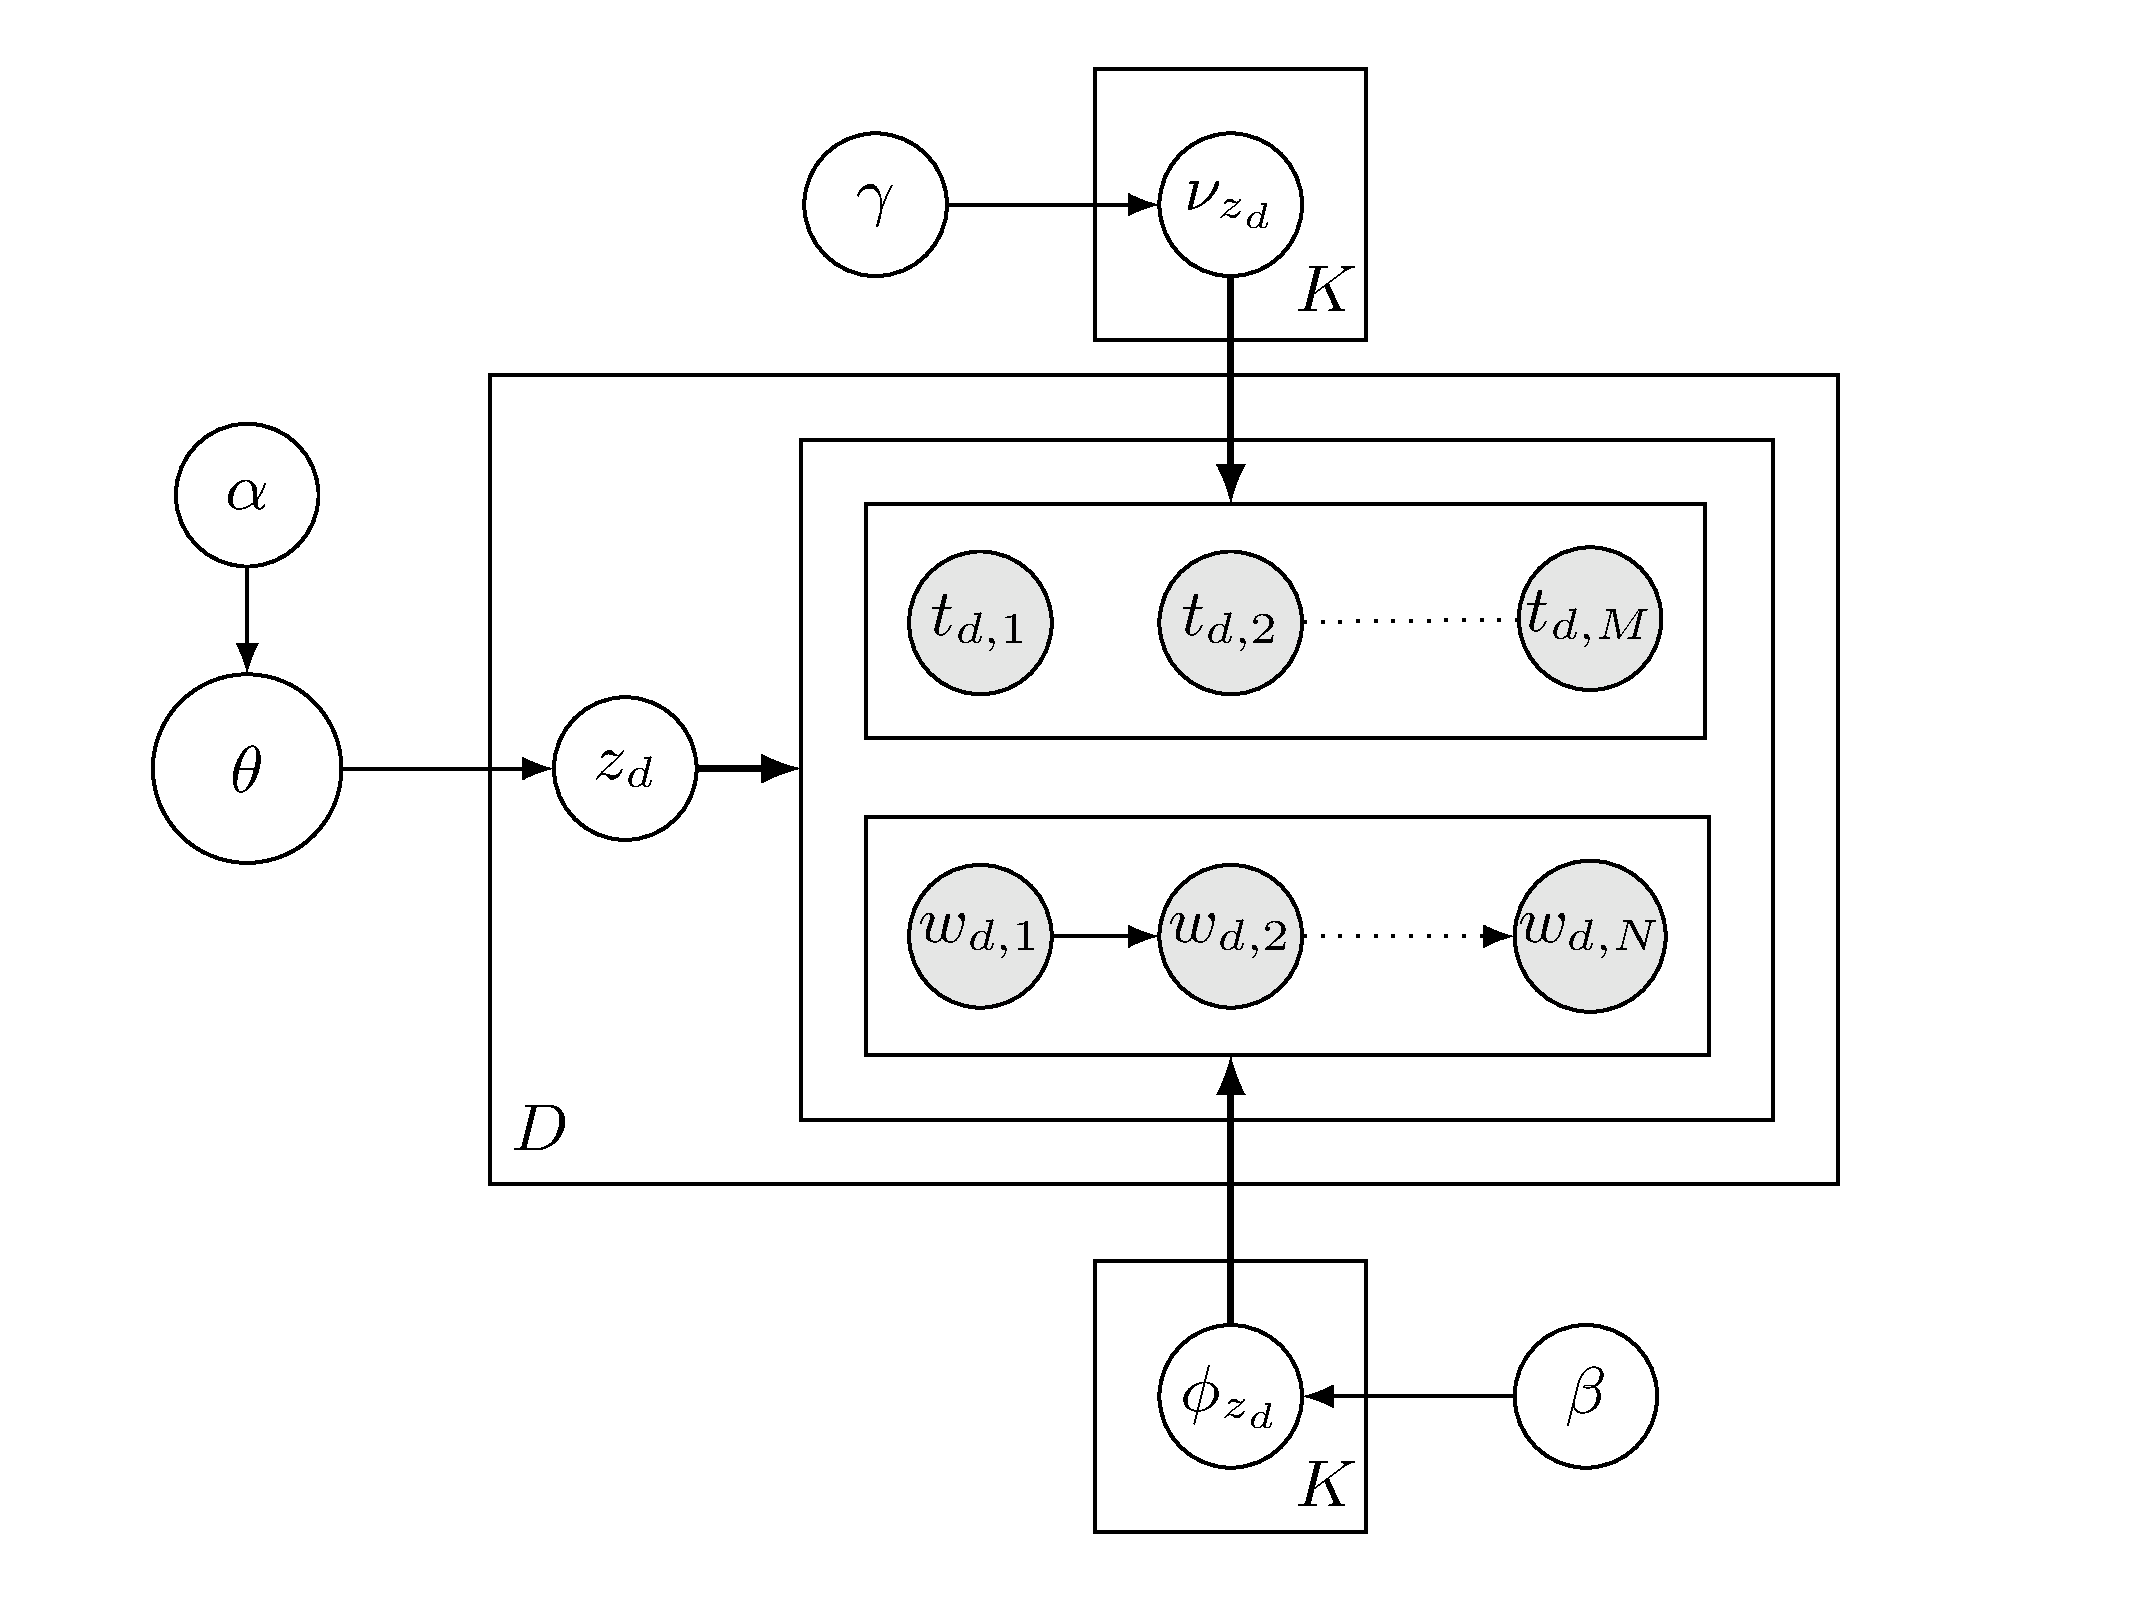
\includegraphics[width=\linewidth]{figures/model.pdf}
\caption{Graphical Model of \ac{ADLTM}. The grey and white circles represent observed and hidden variables, respectively. The plates in the figure mean replicates, with the number of replicates indicated at the bottom of the plate. The plates around the observed sequences represent all unigrams and bigrams in the sequence. }
\label{fig:graphical_model}
\end{figure}

In this probabilistic model $K$ is the number of topics, $D$ is the number of documents, $M$ is the number of unigrams in document $d$, $N-1$ is the number of bigrams in document $d$. In theory, the unigrams and bigrams of this model could be from different vocabularies, so the lengths of the two sequences are not necessarily the same. For instance, if we want to categorise documents not only by sensors but also by time information, we could define hours of timestamps of data points as unigrams instead, thus the discovered topics can take into account time as well. When $t_{d,i}$ and $w_{d,i}$ are the same, $M$ is equal to $N$ and $V$ is equal to $H$. In this simplified scenario, the generative process of \ac{ADLTM} is as specified in \Cref{alg:adl_tm}.

Unlike \acf{LDA} \cite{blei2003latent}, topics are drawn for documents rather than words in this model. The topic $z_d$ of document $d$ is drawn from a multinomial distribution $Mult(\theta)$, where $\theta$ is drawn from a symmetric Dirichlet distribution $Dir(\alpha)$. A unigram $t_{d,i}$ is conditioned on topic $z_d$ and drawn from a multinomial distribution $Mult(\nu_{z_d})$, where $\nu_{z_d}$ is a $H$-dimensional vector drawn from a symmetric Dirichlet distribution $Dir(\gamma)$, and $H$ is the size of the unigram vocabulary. Bigrams are denoted as $w_{d,i} | w_{d,i-1}$ and are also conditioned on the topic $z_d$, so they are drawn from a multinomial distribution $Mult(\phi_{z_d})$ where $\phi_{z_d}$ is a $V \times V$ matrix and $V$ is the vocabulary size of $w_{d,i}$. 

\begin{algorithm}[!t]
    Draw a  $\theta \sim Dir(\alpha)$\;
    \For{$d = 1$ to $D$}
    {
        Draw a topic $\z_d \sim Multi(\theta)$\;
        Draw a $\phi_{z_d} \sim Dir(\beta)$\;
        Draw a $\nu_{z_d} \sim Dir(\gamma)$\;
        \For{$n = 1$ to $N$}
        {
            Draw a unigram $t_{d,n} | z_d  \sim Mult(\nu_{z_d})$\;
            \uIf{$n > 1$}
            {
                Draw a bigram $w_{d,n} | w_{d,n-1}, z_d  \sim Mult(\phi_{z_d})$\;
            }
        }
    }
 \caption{Generative Processes of \ac{ADLTM}}
 \label{alg:adl_tm}
\end{algorithm}

\subsection{Gibbs Sampling of \ac{ADLTM}}
An effective approximation approach to inference in topic models is Gibbs sampling  \cite{rosen2004author,griffiths2004finding}, which is one of the most popular \acl{MCMC} algorithms. The core idea of Gibbs sampling is to construct the Markov chain by drawing each latent variable from their conditional distribution in turn. In Gibbs sampling of \ac{ADLTM}, the conditional probability of topic $z_d$ can be estimated as follows:
%
\begin{equation} \label{eqa1}
\begin{split}
P(z_d|\z_{-d},\w, \tb) \propto \ & P(z_d|\z_{-d}) P(w_d|z_d,\z_{-d},\w_{-d}) \\
& \times P(t_d|z_d,\z_{-d},\tb_{-d})
\end{split}
\end{equation}
%
where $\z_{-d}$ represents topics assigned to all documents except document $d$, $\tb_{-d}$ and $\w_{-d}$ are unigram and bigram sequences of all other documents except document $d$. As a topic is drawn for each document, the joint probability of topics of all documents can be calculated by:
%
\begin{equation} \label{eq:dmclda2}
\begin{split}
P(\z) & = P(z_1) P(z_2) \cdot\cdot\cdot P(z_D),
\end{split}
\end{equation}
%
Since $\z_d \sim Multi(\theta)$ and $\theta \sim Dir(\alpha)$, the first term of \Cref{eqa1} can be estimated by:
%
\begin{equation} \label{eq:dmclda3}
\begin{split}
P(z_d = k|\z_{-d}) & \propto C_k^{-} + \alpha
\end{split}
\end{equation}
%
where $C_k^-$ is the number of documents assigned to topic $k$ except current document $d$.


As all words in a document are drawn from one topic, the full conditional probability of the bigram sequence $w_d$ can be estimated by \Cref{eq:dmclda6}, where 
$I(x)$ is the indicator function; 
$w_{d,n}$ is the $n^{\mathrm{th}}$ word in the bigram sequence of document $d$; 
$C_{w_{ijk}}^-$ is the number of times word $j$ is followed by word $i$ in topic $k$, except in current document $d$; and 
$C_{w_{*jk}}^-$ is the number of times word $j$ followed by any word in topic $k$, except in current document $d$. 
%
\begin{equation} \label{eq:dmclda6}
\begin{split}
P&(w_{d}  | z_d = k, \z_{-d},\w_{-d}) \\  
&= \prod_{n=2}^{N} P(w_{d,n} | w_{d,n-1}, z_d = k, \z_{-d},\w_{-d}) \\ 
&\propto \prod_{n=2}^{N} \left( \sum_{j=1}^{V} \frac{\sum_{i=1}^{V}(C_{w_{ijk}}^{-} + \beta)I(w_{d,n} = i)}{C_{w_{*ju}} ^{-}+ V\beta} I(w_{d,n-1} = j) \right)
\end{split}
\end{equation}

\newcommand{\tf}{\ensuremath{\mathit{tf}}}
\newcommand{\idf}{\ensuremath{\mathit{idf}}}
An important characteristic of the sensor data is that most transitions between sensors are self-transitions. If we want to estimate the probability of transitions between different sensors in an activity, which is the purpose of introducing bigrams, the weights of self-transitions should be decreased in probability estimation. A common approach in natural language processing is to use \tf-\idf\ \cite{salton1988term} as the weight of each individual word. \tf\ indicates term frequency which is simply defined as the number of times a word appears in the dataset. \idf\ refers to the inverse document frequency, where the document frequency is the number of documents that contain this word. When the term frequency is much higher than the document frequency, \tf-\idf\ is still dominated by term frequency, so in this case we deployed \textbf{document frequency} for counting bigrams in \Cref{eq:dmclda6}.

Similarly, all the unigrams in document $d$ are drawn together too, so the conditional probability of $t_d$ is given by:
%
\begin{equation} \label{eq:adl_tm1}
\begin{split}
P(t_d | z_d,\z_{-d}, \tb_{-d}) & = \prod_{n=1}^{M} P(t_{d,n}  | z_d = k, \z_{-d}, \tb_{-d}) \\
& \propto \prod_{n=1}^{M} \left( \sum_{h=1}^H \frac{(C_{t_{hk}}^{-}+\gamma)}{(C_{t_{*k}}^{-}+H\gamma)} I(t_{d,n} = h) \right)
\end{split}
\end{equation}
%
where $C_{t_{hk}}^{-}$ is the number of times the unigram $h$ has been assigned to topic $k$, except in document $d$; and 
$C_{t_{*k}}^{-}$ is the number of times that any unigram has been assigned to topic $k$, except in document $d$. Here, unlike for bigrams, the counts of unigrams are counted by \textbf{term frequency}.

Using \Cref{eq:dmclda3,eq:dmclda6,eq:adl_tm1}, the probability $P(z_d | z_{-d}, \w, \tb)$ (\Cref{eqa1}) can be calculated by Gibbs sampling and subsequently the parameters $\theta$, $\phi$, $\nu$ of \ac{ADLTM} can be estimated.

%\input{sections/05_results}
\section{Experimental Evaluation}
\label{sec:eva}

%\setlength{\tabcolsep}{0.5em} % for the horizontal padding
{%\renewcommand{\arraystretch}{1.2}% for the vertical padding
\begin{table}[!b]
\centering
\scriptsize
\begin{tabular}{ccccc}
\toprule
 Dataset & \# Activities & \# Binary Sensors & Duration (days) & \# Residents \\
\midrule
hh122       & 32 & 24 & 30 & 1     \\
hh120      & 32 & 24 & 64 & 1     \\
milan   & 15 & 31 & 31 & 1+pet \\
\bottomrule
\end{tabular}
\caption{Properties of Datasets}
\label{tab:raw2}
\end{table}
}

We have tested our approach on several CASAS datasets which were collected in real smart homes. 
The properties of datasets \textit{hh122}, \textit{hh120} \cite{cook2013casas} and \textit{milan} \cite{cook2009assessing} are listed in \Cref{tab:raw2}. 
These datasets are partially annotated with activities, so this gives us an opportunity to compare the results of our unsupervised model with the annotations. 
All test results in this section are produced with the following hyperparameters:
\begin{enumerate}
\item Topic prior: $\alpha = 50 / K$;
\item Bigram and unigram priors: $\beta = 5 / V$, $\gamma = 5 / H$.
\end{enumerate}
The number of topics $K$ is guaranteed larger than the number of locations and selected by several tests, because we assume there are more types of activities than locations. However, if $K$ is too large there will be empty topics (which are not assigned any document) after convergence. For instance, there are 9 locations of dataset hh122, so $K$ is experimentally set to 12. 
The number of iterations of Gibbs sampling is 50.

\subsection{Evaluation of Discovered Topics}

\begin{figure}[!t]
\begin{subfigure}{0.32\linewidth}
    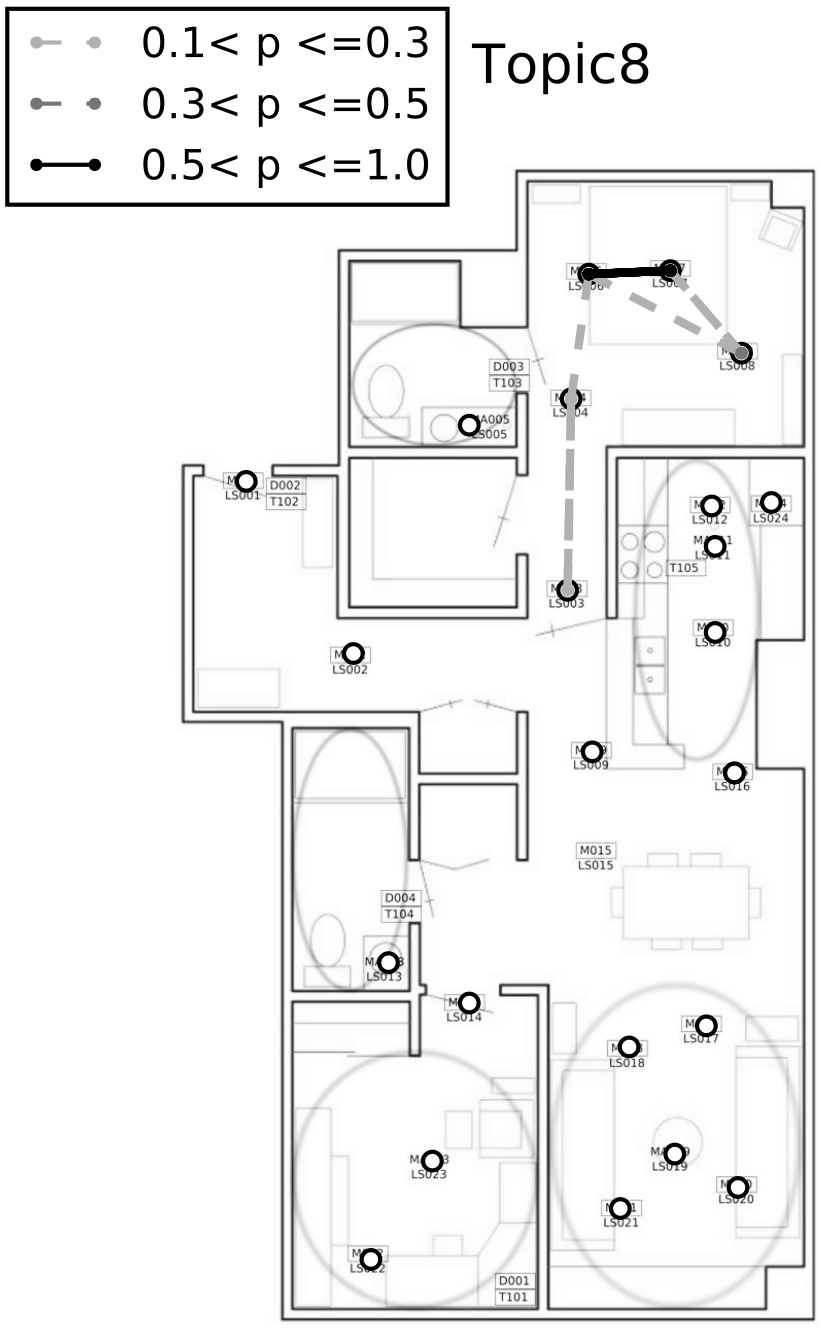
\includegraphics[width=\linewidth]{figures/adl_tm/topic8_bw_cp}
    \caption{topic 8}
    \label{fig:adl_tm-8}
\end{subfigure}
\begin{subfigure}{0.32\linewidth}
    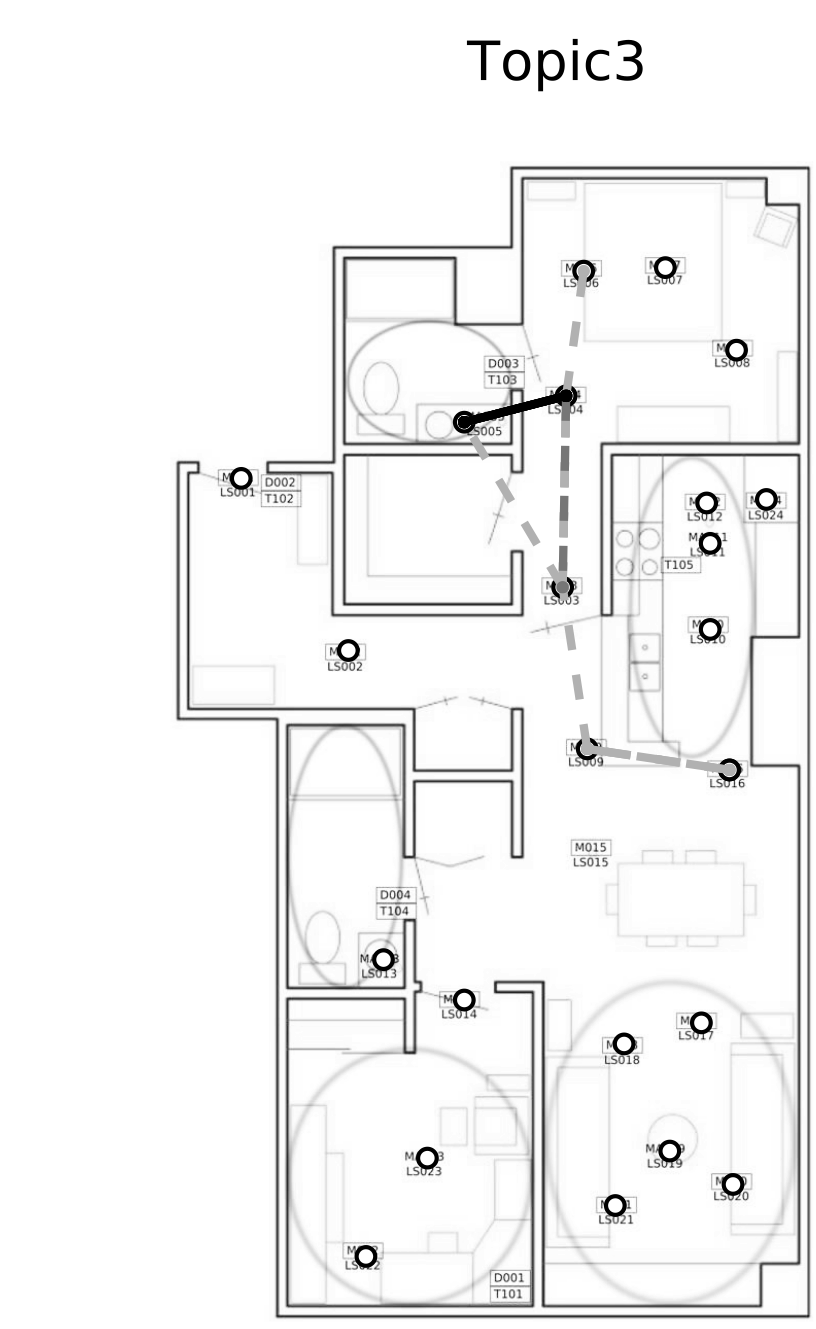
\includegraphics[width=\linewidth]{figures/adl_tm/topic3_bw_cp}
    \caption{topic 3}
    \label{fig:adl_tm-3}
\end{subfigure}
\begin{subfigure}{0.32\linewidth}
    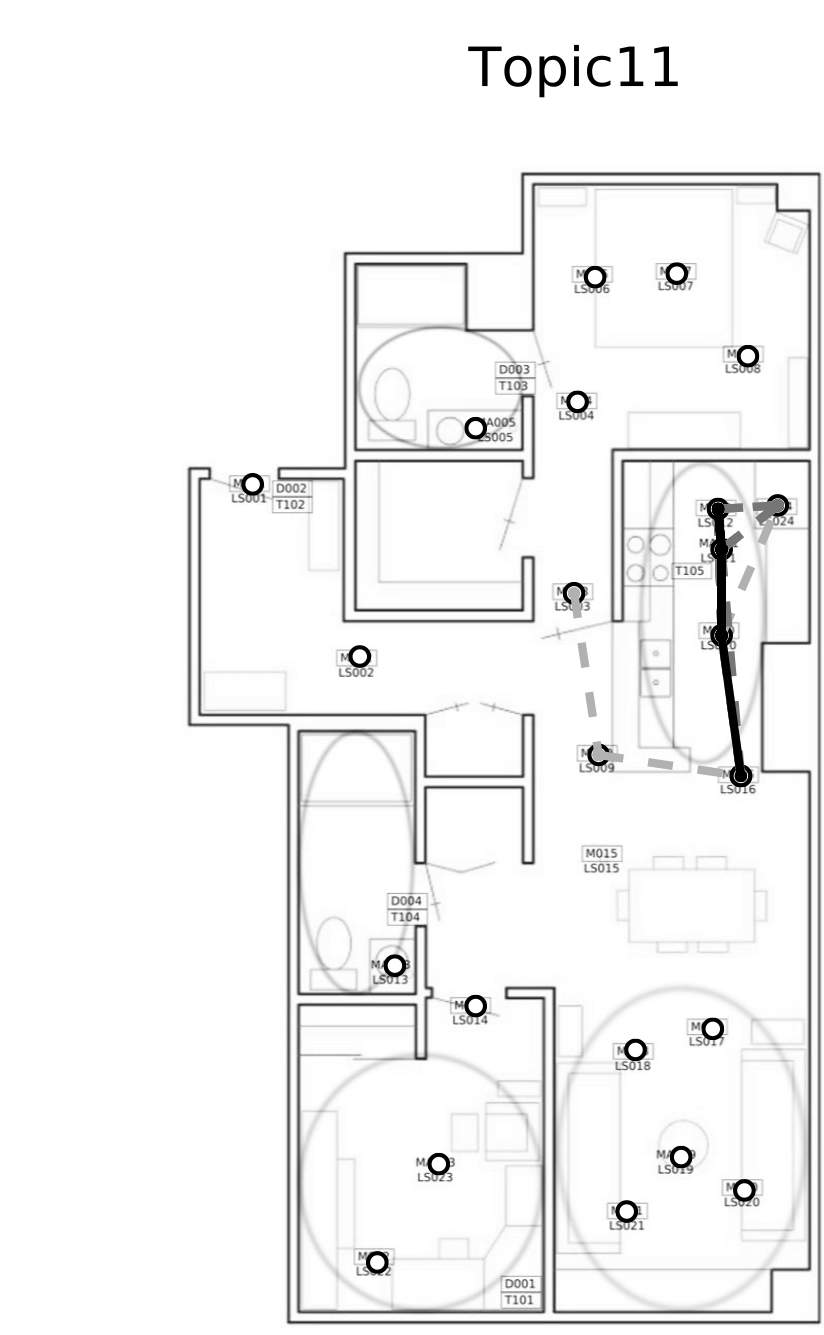
\includegraphics[width=\linewidth]{figures/adl_tm/topic11_bw_cp}
    \caption{topic 11}
    \label{fig:adl_tm-11}
\end{subfigure}
\caption{Topics discovered by \ac{ADLTM} in dataset hh122. The small circles represent installed binary sensors; black dots and lines represent highly probable sensor activations and transitions within a topic.}
\label{fig:adl_tm}
\end{figure}

\begin{figure}[!b]
\begin{subfigure}{0.32\linewidth}
    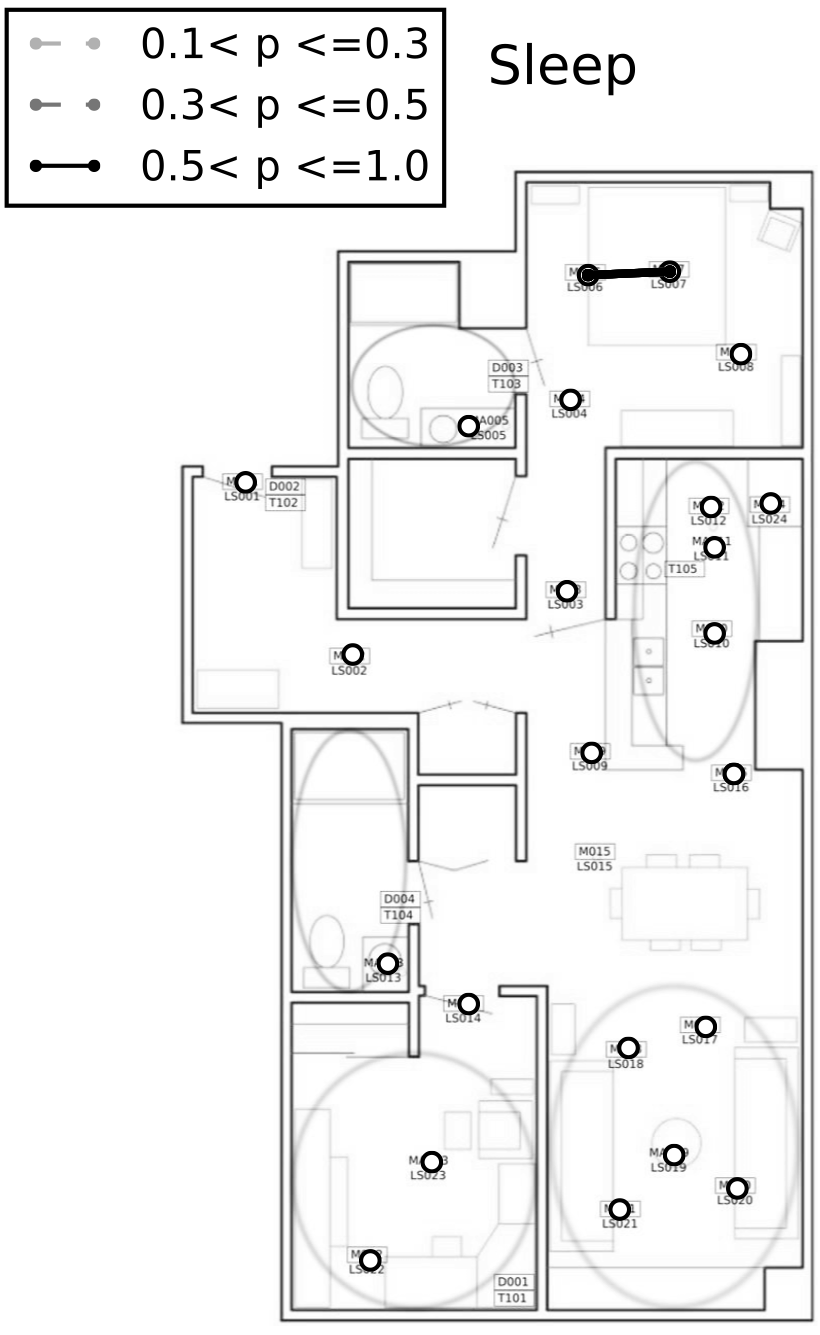
\includegraphics[width=\linewidth]{figures/visActs/Sleep_bw_cp}
    \caption{Sleep}
\end{subfigure}
\begin{subfigure}{0.32\linewidth}
    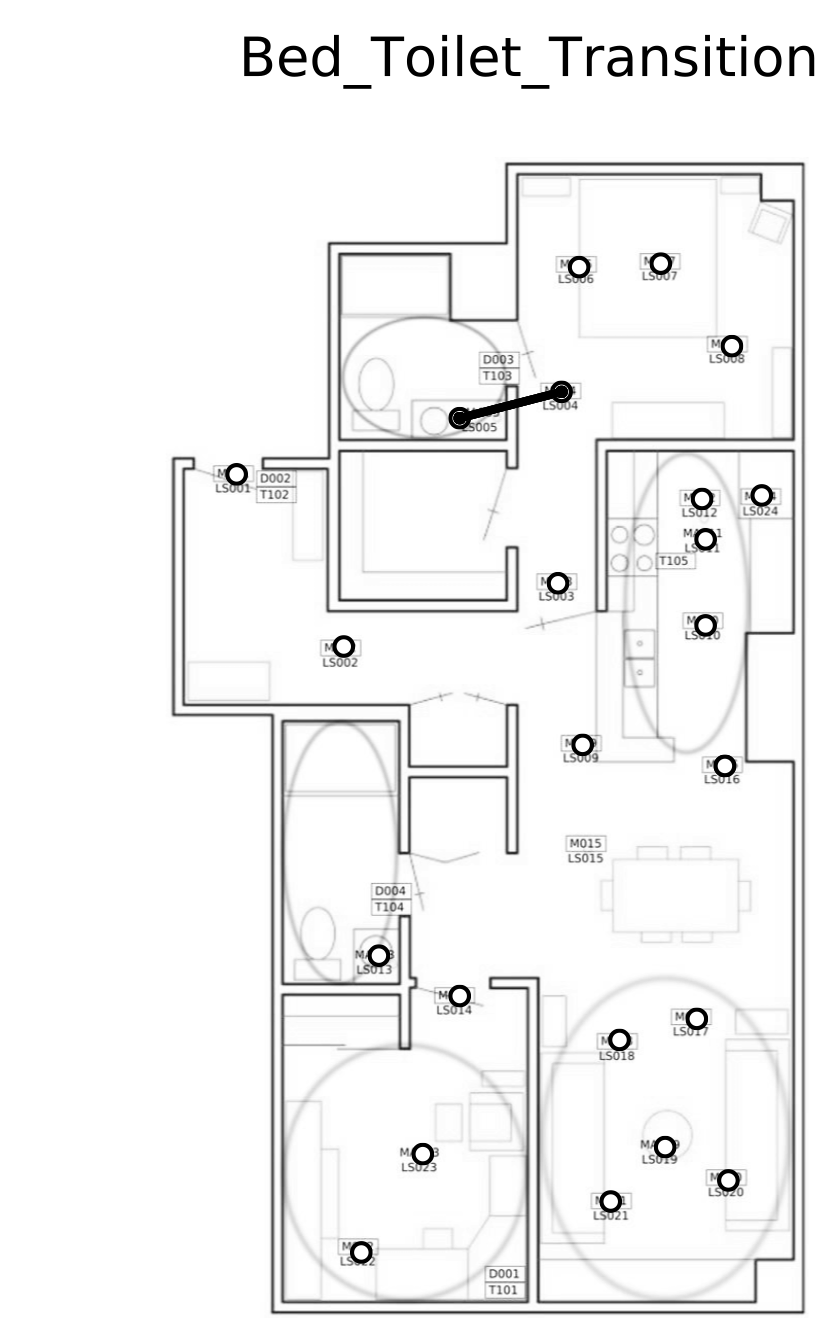
\includegraphics[width=\linewidth]{figures/visActs/Bed_Toilet_Transition_bw_cp}
    \caption{Bed-to-Toilet}
\end{subfigure}
\begin{subfigure}{0.32\linewidth}
    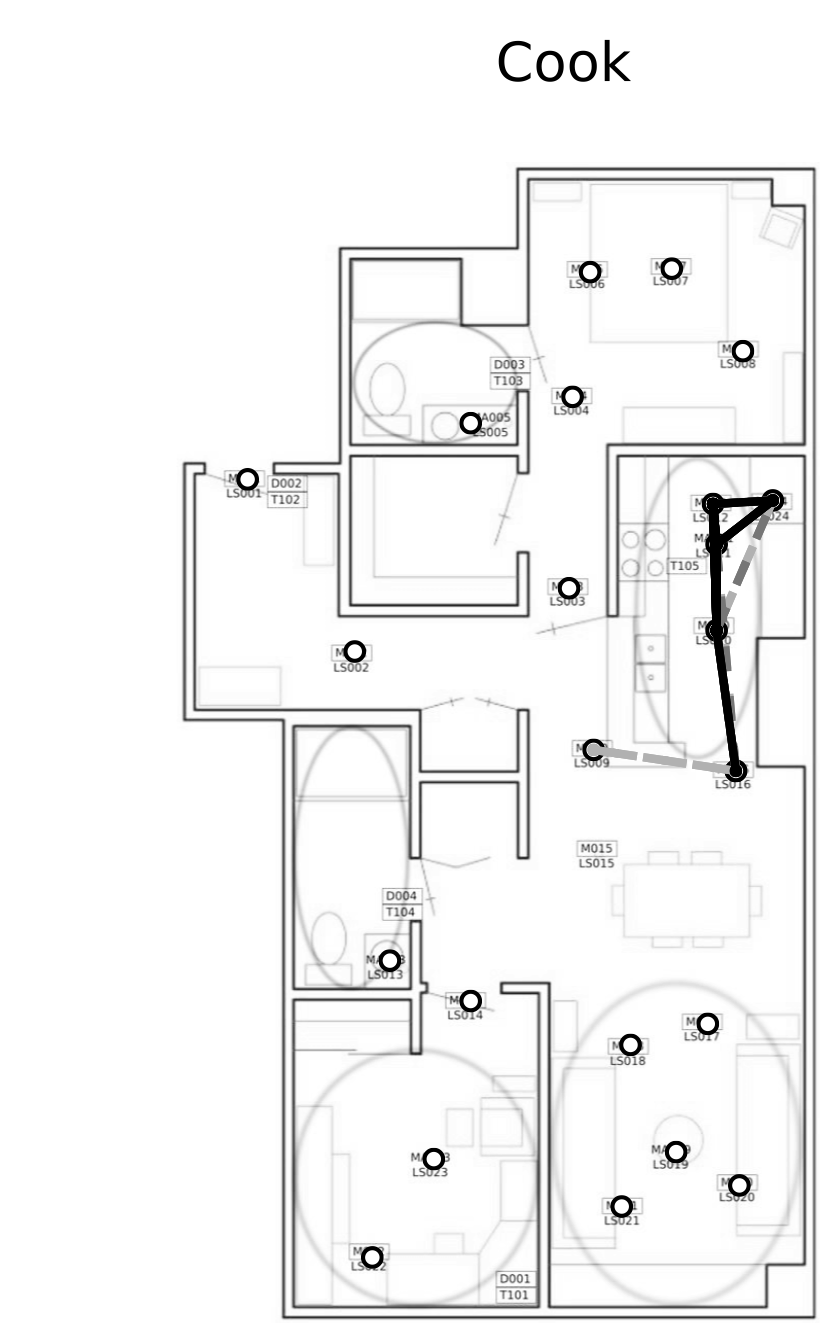
\includegraphics[width=\linewidth]{figures/visActs/Cook_bw_cp}
    \caption{Cook}
\end{subfigure}
\caption{Some annotated activities in dataset hh122.}
\label{fig:visacts}
\end{figure}

To understand what hidden patterns have been discovered by \ac{ADLTM}, we have visualised the discovered topics. As illustrated in \Cref{fig:adl_tm},  the most frequently activated sensors and transitions of a topic (the black dots and lines) only appear in one location. This phenomenon matches the actual activities, which mostly occur in a specific location of the house: for example, ``Sleep'' occurs in the bedroom and ``Cook'' occurs in the kitchen. Although some sensors of neighbouring locations are also involved, they are much less frequent in that topic (grey dots and lines).
%
Compared with the annotated activities (\Cref{fig:visacts}), these discovered topics are similar but somewhat less concentrated in an area. 

To evaluate the similarity between discovered topics and annotated activities, we adopted the \ac{FM} Index \cite{fowlkes1983method,Ramirez2012125}, a variant of the $F_1$ score adapted for clustering, to measure the discovered topics quantitatively. The results on three datasets are shown in \Cref{tab:fmidx}, which indicates \ac{ADLTM} outperforms \ac{LDA} \cite{blei2003latent} and \ac{BTM} \cite{wallach2006topic} in this criterion.

%\setlength{\tabcolsep}{0.5em} % for the horizontal padding
{%\renewcommand{\arraystretch}{1.2}% for the vertical padding
\begin{table}[!t]
\centering
\scriptsize
\begin{tabular}{lccc}
\toprule
              & hh122  & hh120  & milan \\
\midrule
Random topics & 0.0798 & 0.0969 & 0.1193 \\
\ac{BTM}      & 0.1515 & 0.1988 & 0.3225 \\
\ac{LDA}      & 0.3268 & 0.3486 & 0.5634 \\
\ac{ADLTM}    & 0.3362 & 0.4072 & 0.6190 \\
\bottomrule
\end{tabular}
\caption{\ac{FM} Index of topics by different methods}
\label{tab:fmidx}
\end{table}
}


\subsection{Evaluation of Segmentation}
Another thing worth evaluating is the segmentation by topics. After the documents have been categorised by topics, new segments of the data sequence are generated. Some adjacent documents assigned to the same topic have been merged together and become a new segment now.  In the ideal case, each segment of topics should correspond to one occurrence of the resident's daily activities. We evaluate the segmentation by several metrics as described in this section.

\Cref{fig:visseg} displays segmentation by activities, topics and documents. They are visualised with one day's data. The discovered topics integrate some documents so that the segments become less trivial but meanwhile additional error might occur due to the integration. 

\begin{figure}[!b]
\centering
\begin{subfigure}{0.48\linewidth}
    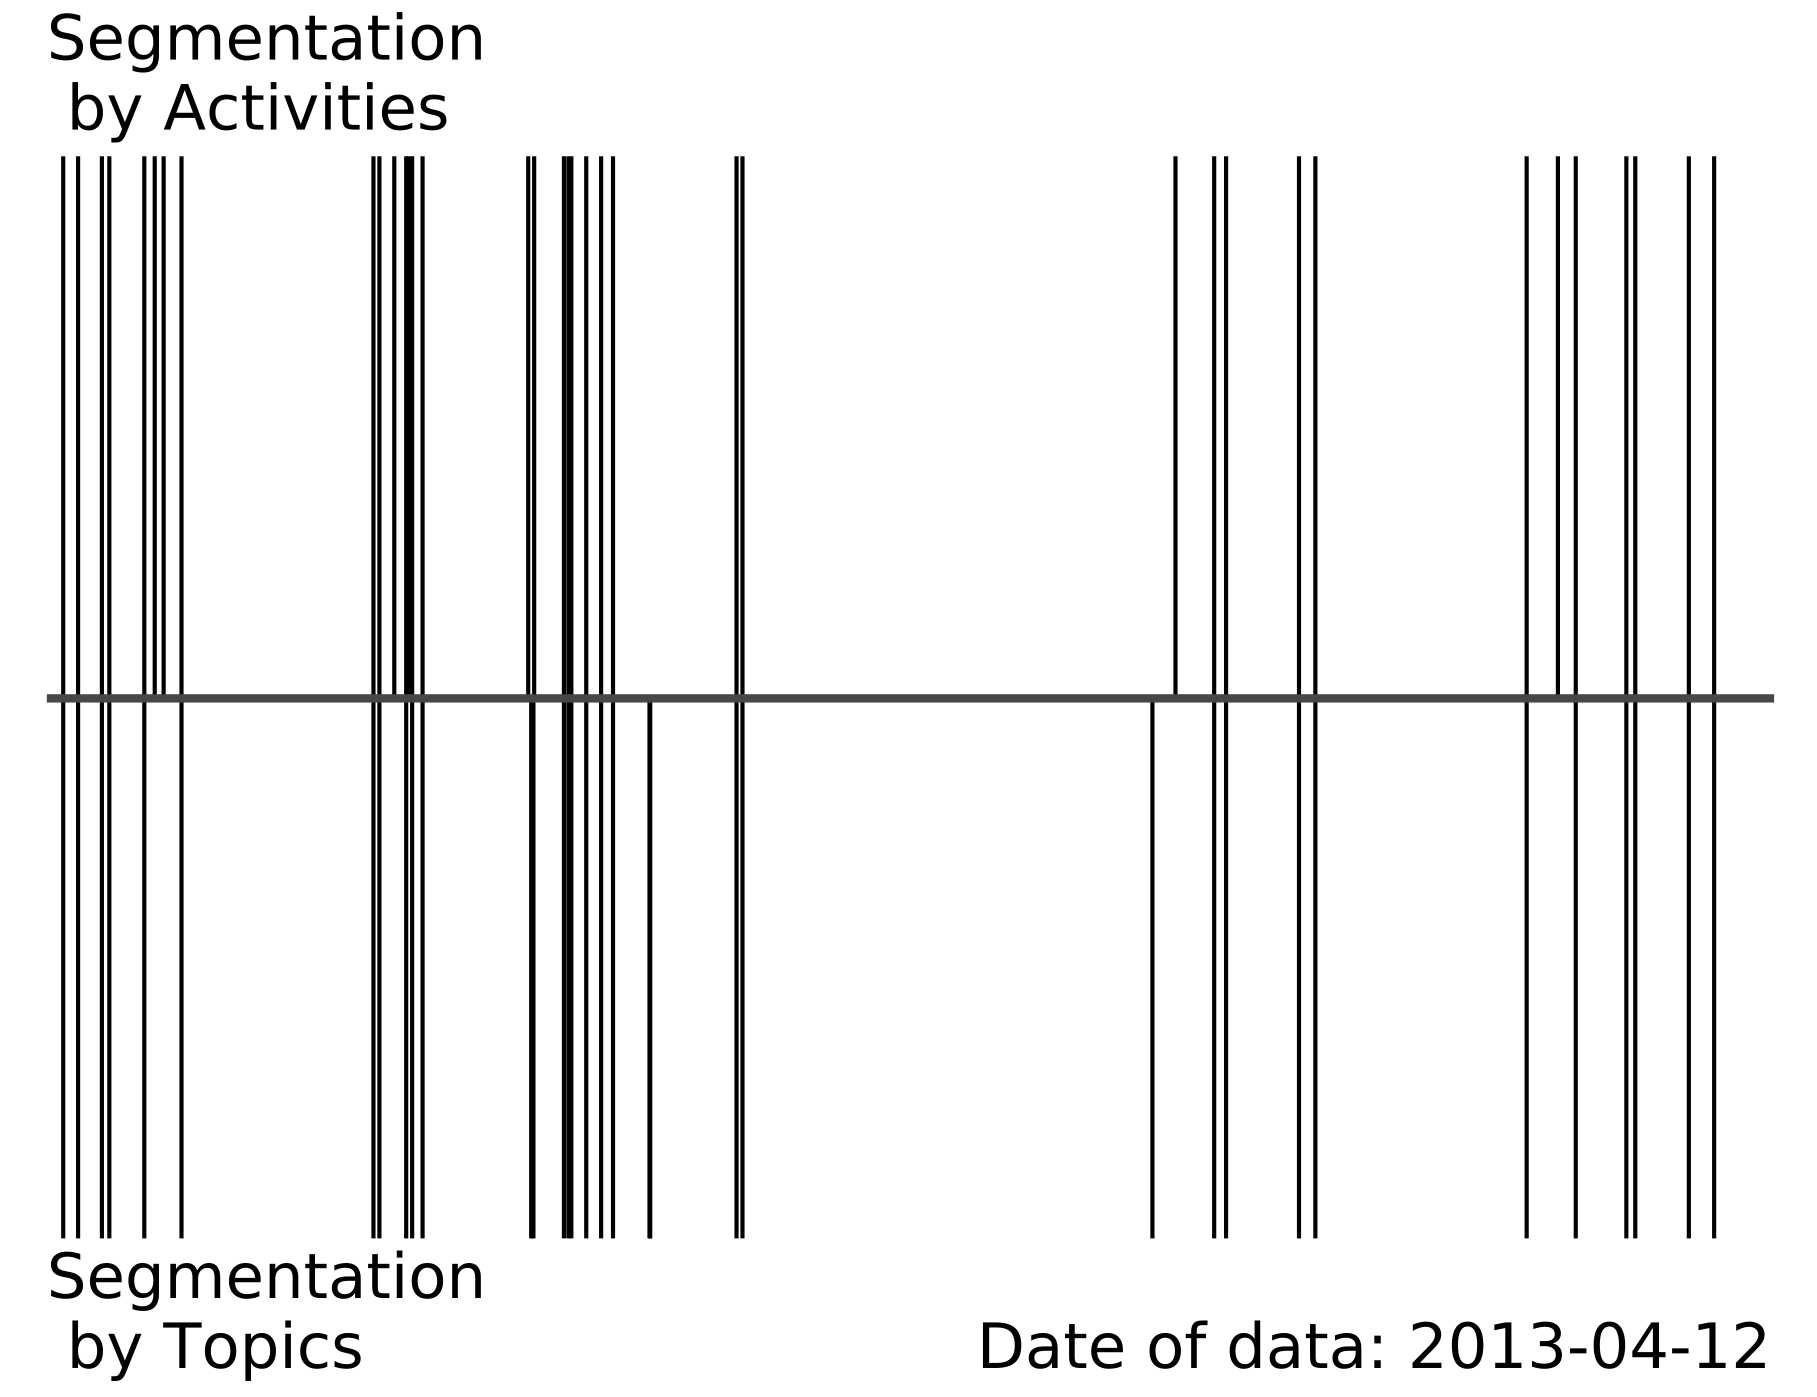
\includegraphics[width=\linewidth]{figures/adl_tm/act_topic_segs_sub1_bw_cp}
    \caption{Segmentation by topics and activities}
\end{subfigure} \ \ 
\begin{subfigure}{0.48\linewidth}
    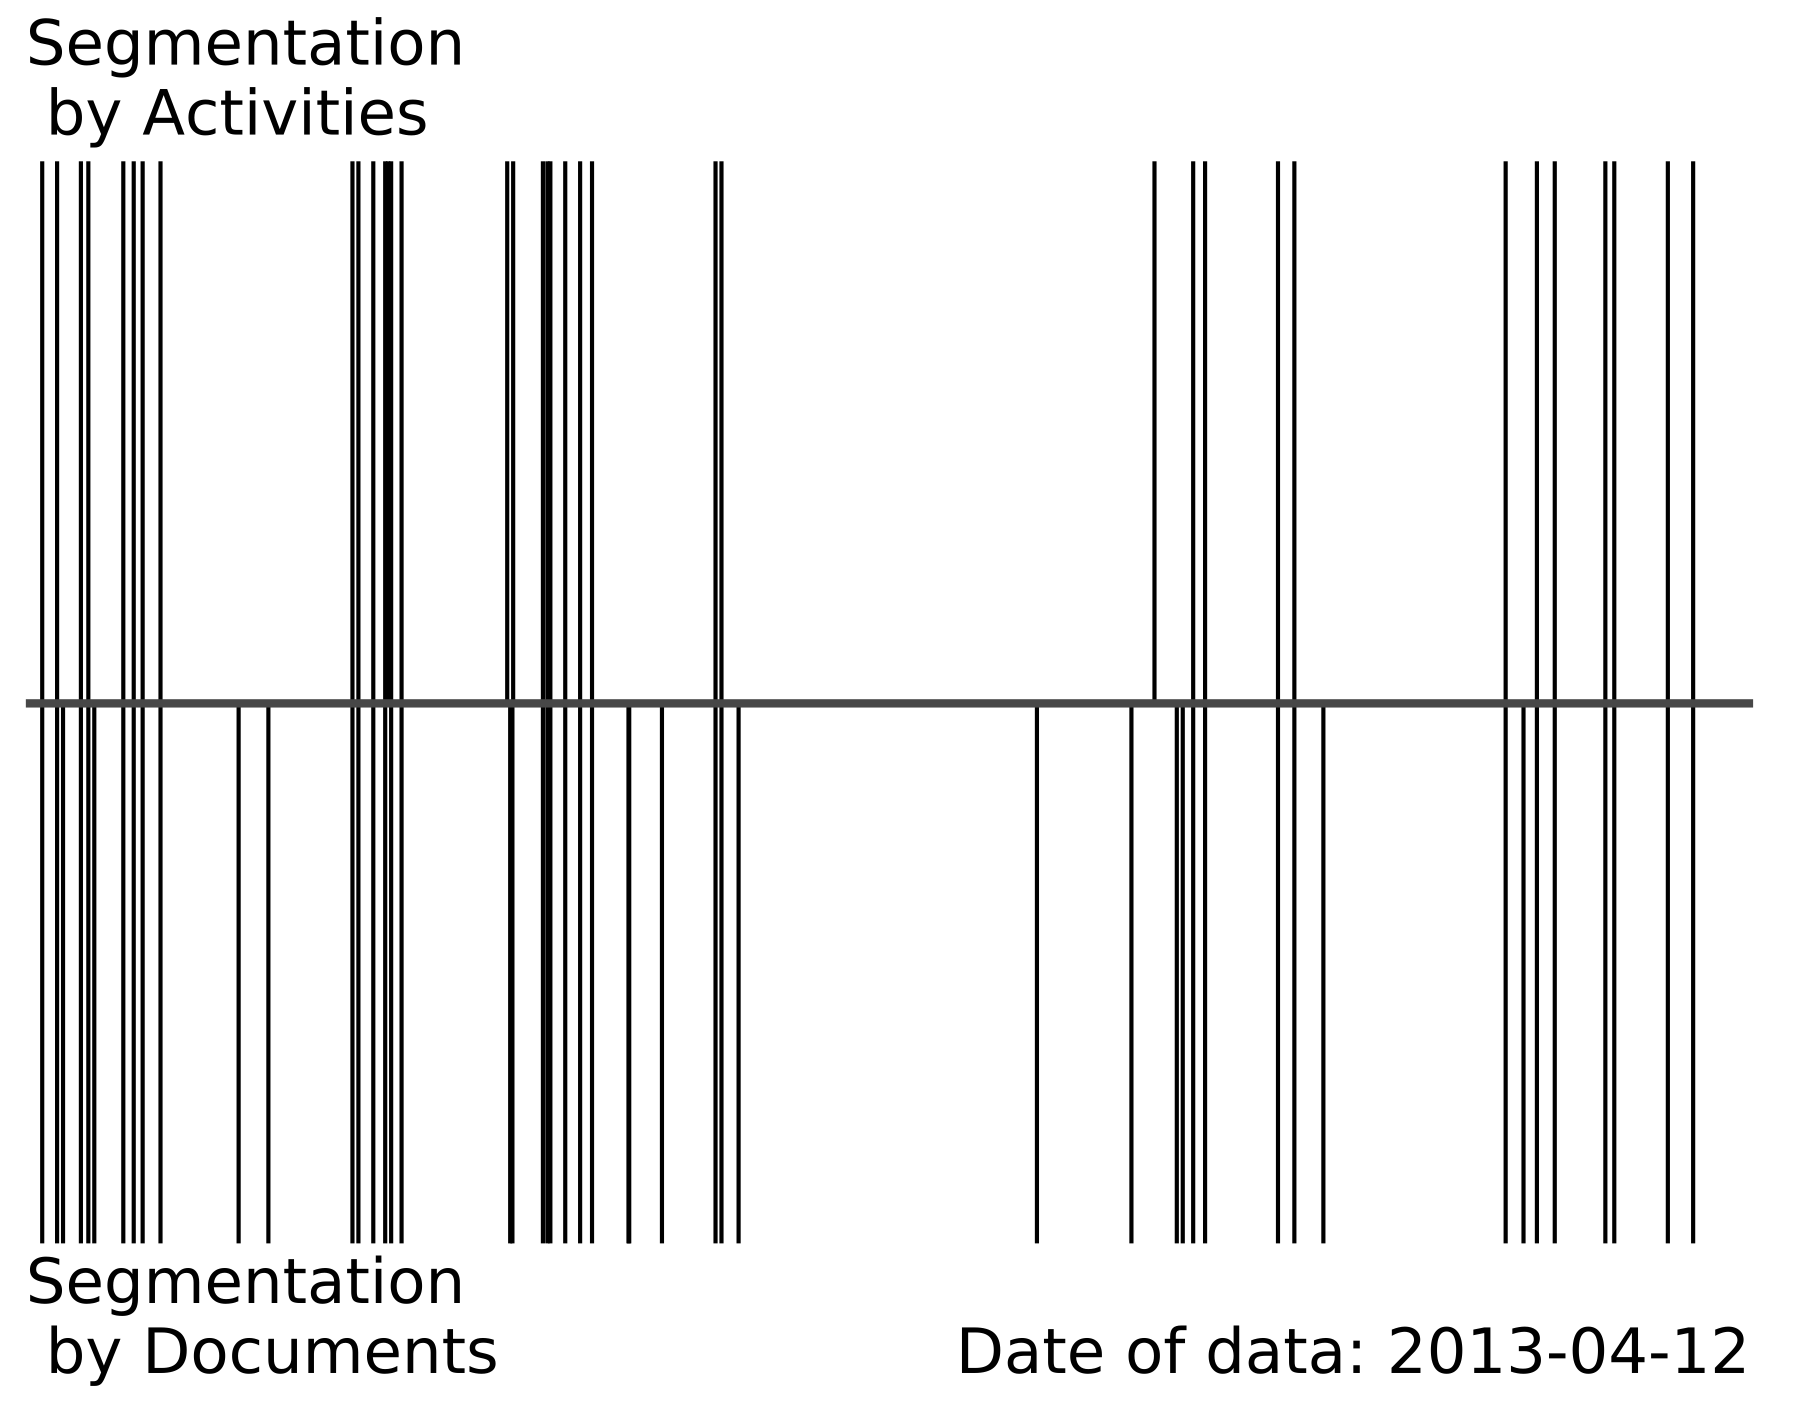
\includegraphics[width=\linewidth]{figures/adl_tm/act_doc_segs_sub1_bw_cp}
    \caption{Segmentation by documents and activities}
\end{subfigure}
\caption{Visualisation of segmentation by \ac{ADLTM} (dataset: hh122). The upper half of a sub-figure is the segmentation by activities, lower half is by topics (a) or documents (b). The date at the bottom right is the date when the data was generated.}
\label{fig:visseg}
\end{figure}

\newcommand{\fracii}[2]{\ensuremath{#1/#2}}
We have defined two criteria to evaluate the segmentation quantitatively:
\begin{enumerate}
\item  \textbf{Segmentation Error}, which is the average error over all segments of the data sequence:
\begin{equation*} %\label{eq:eqa1}
Err_{s} = \frac{\sum_i^{D_{s}} E_{i}}{N_{dp}}
\end{equation*}
%
where $D_s$ is the number of generated segments in the data sequence; 
$N_{dp}$ is the total number of data points; and 
$E_i$ is the number of data points in segment $i$ who do not belong to the dominant activity of this segment, which can be calculated as
% \Cref{eq:seg2}:
\begin{equation*} \label{eq:seg2}
\begin{split}
E_i &= N_i - \sum_{j=1}^{N_i} I(a_{ij} = m),\ \ \
m = \argmax_k(\sum_{j=1}^{N_i} I(a_{ij} = k))
\end{split}
\end{equation*}
Here, $N_i$ denotes the number of data points in segment $i$; 
$a_{ij}$ is the annotated activity of data point $j$ in segment $i$; 
$I(x)$ is the indicator function; 
$m$ is the activity that has maximum number of data points in segment $i$. 
\item \textbf{Fragment Ratio}, which is the average number of segments in one occurrence of an activity:
\begin{equation*} %\label{eq:eqa2}
R_{fr} = \frac{D_{s}}{D_{a}}
\end{equation*}
where 
% $D_s$ is the same as in \Cref{eq:eqa1}, 
$D_{a}$ is the number of occurrences of activities in the evaluated data. 
\end{enumerate}
The segmentation by actual activities is viewed as the ideal result with segmentation error zero and fragment ratio one. 

\Cref{tab:cpmr} gives the evaluation results of segmentation by different methods tested on three datasets. 
The documents are generated by the algorithm described in \Cref{alg:segmentation}. As we can see, the documents have lower segmentation errors and higher fragment ratio than the topic models, because most of the documents are much smaller than segments of activities or topics. The topic models decrease the fragment ratio by integrating trivial documents but increase the segmentation error. 
The results show that \ac{ADLTM} outperforms \ac{LDA} \cite{blei2003latent} and the \ac{BTM} \cite{wallach2006topic} in both criteria.

%\setlength{\tabcolsep}{0.5em} % for the horizontal padding
{%\renewcommand{\arraystretch}{1.2}% for the vertical padding
\begin{table}[!b]
\centering
\scriptsize
\begin{tabular}{lcccccc}
\toprule
\multirow{2}{*}{} & \multicolumn{2}{c}{hh122} & \multicolumn{2}{c}{hh120} & \multicolumn{2}{c}{milan} \\ \cmidrule(l){2-7} & $Err_s$     & $R_{fr}$     & $Err_s$     & $R_{fr}$   & $Err_s$     & $R_{fr}$     \\
\midrule
%Activities          & 0.0000 & 1.000 & 0.0000 & 1.000 & 0.0000 & 1.000 \\
Documents           & 0.0197 & 1.596 & 0.0404 & 2.084 & 0.0342 & 1.563 \\
\ac{LDA}            & 0.0541  & 1.178 & 0.0531 & 1.554 & 0.0409 & 1.157 \\
\ac{BTM}            & 0.0619  & 1.174 & 0.0568 & 1.853 & 0.0428 & 1.394 \\
\ac{ADLTM}          & 0.0512  & 1.102 & 0.0516 & 1.364 & 0.0406 & 1.149 \\
\bottomrule
\end{tabular}
\caption{Evaluations of Segmentations}
\label{tab:cpmr}
\end{table}
}

The topic segmentation is based on the document segmentation, so the parameter $t_{th}$ of the segmentation algorithm (\Cref{alg:segmentation}) can affect the segmentation results of topic models as well. When $t_{th}$ is smaller, the segmentation error is lower, the fragment ratio is higher and {\em vice-versa}, resulting in a trade-off between the two criteria when choosing this parameter. Hence in practical cases some prior knowledge about the minimum duration of activities will help to improve the segmentation results.

\subsection{Applications}
After the documents have been categorised by topics the data sequence is fully segmented and a new data space can be constructed by generating one data point for each segment with 3 features: the start time-stamp of its segment, the duration and the topic of this segment. 
By this transformation, the raw data space is highly compressed without losing important information: for instance, the dataset hh122 is compressed from 129\,936 to 2\,792 data points. Based on the compressed data space, we can perform various further analyses to leverage information contained in the discovered topics.

As can be seen in the visualisation of topic 8 (\Cref{fig:adl_tm-8}), we can assume that it represents the bedroom activities, so now we visualise all the segments assigned to topic 8 as in \Cref{fig:vissleep-a}. The data points with duration larger than 1 hour are mostly distributed between 10 PM to 7 AM, which indicates the regular sleeping time of the resident during night. We can also easily calculate the average sleeping duration of this resident as 7.02 hours. When combined with the distribution of topic 3 (\Cref{fig:adl_tm-3}), we can infer that the resident usually needs to use the toilet 3 times per night during sleep. \Cref{fig:vissleep-b} plots the annotated activity ``Sleep''. These two figures are very similar, which indicates that the discovered topic 8 successfully represents the activity ``Sleep''. 
%
 \begin{figure}[!t]
 \centering
\begin{subfigure}{0.49\linewidth}
    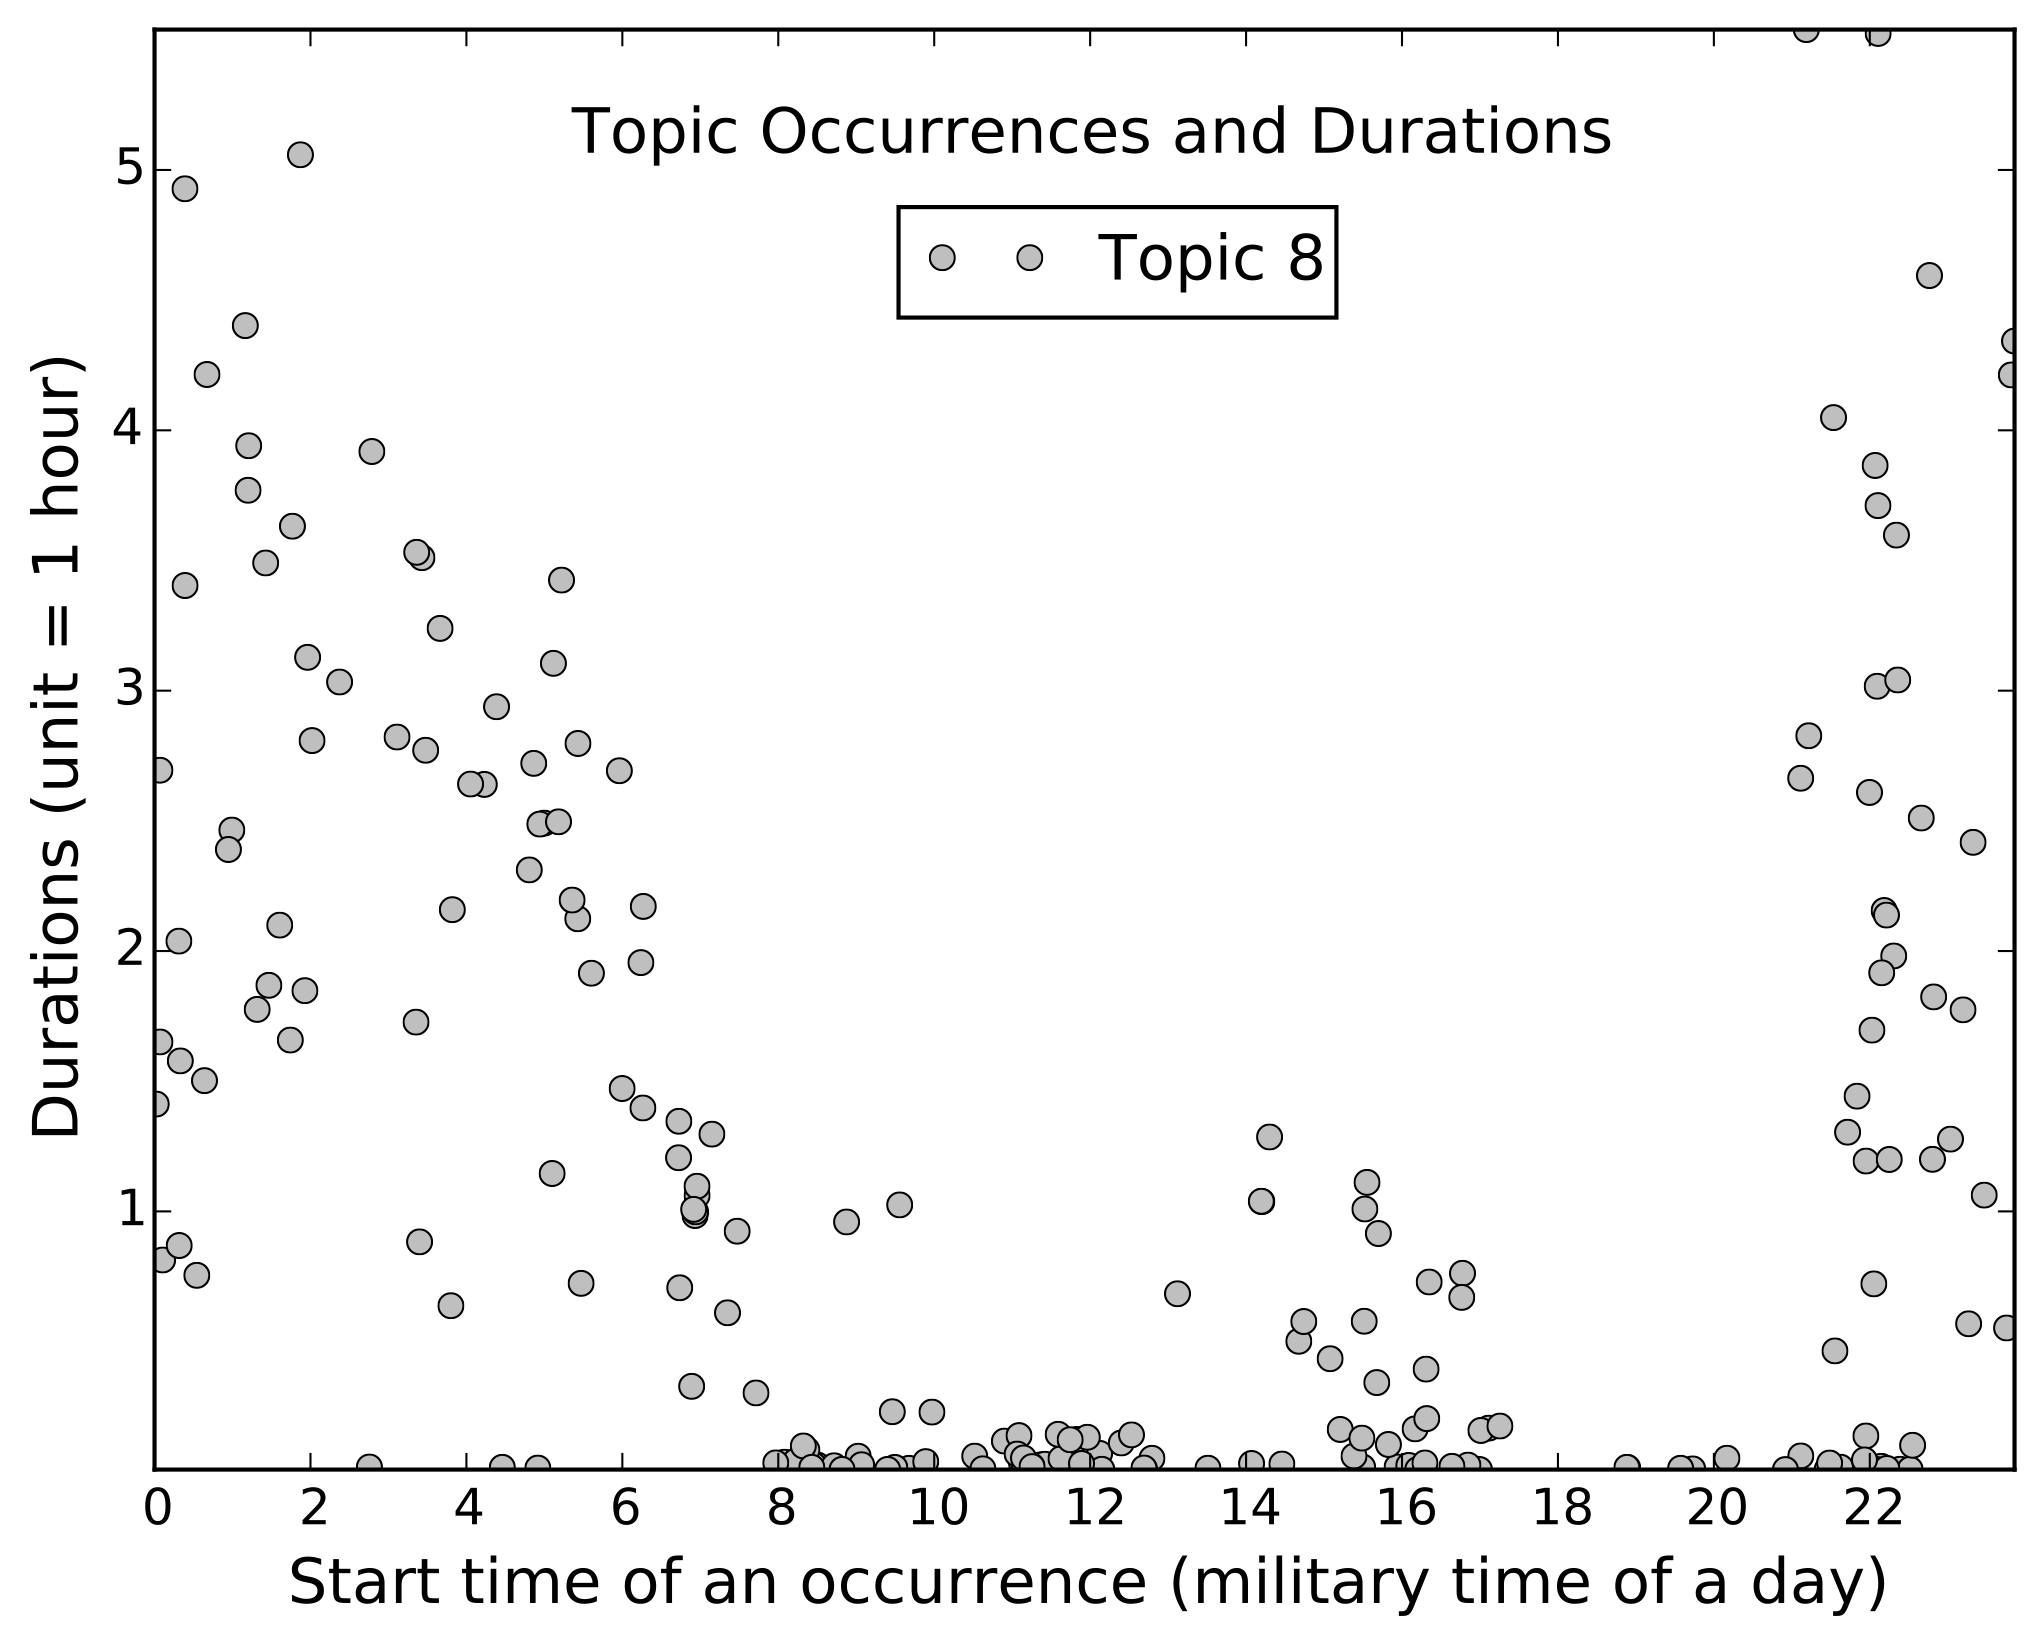
\includegraphics[width=\linewidth]{figures/adl_tm/Topic_time_stat_sleep_bw}
    \caption{Distribution of Topic 8}
    \label{fig:vissleep-a}
\end{subfigure} \
\begin{subfigure}{0.49\linewidth}
    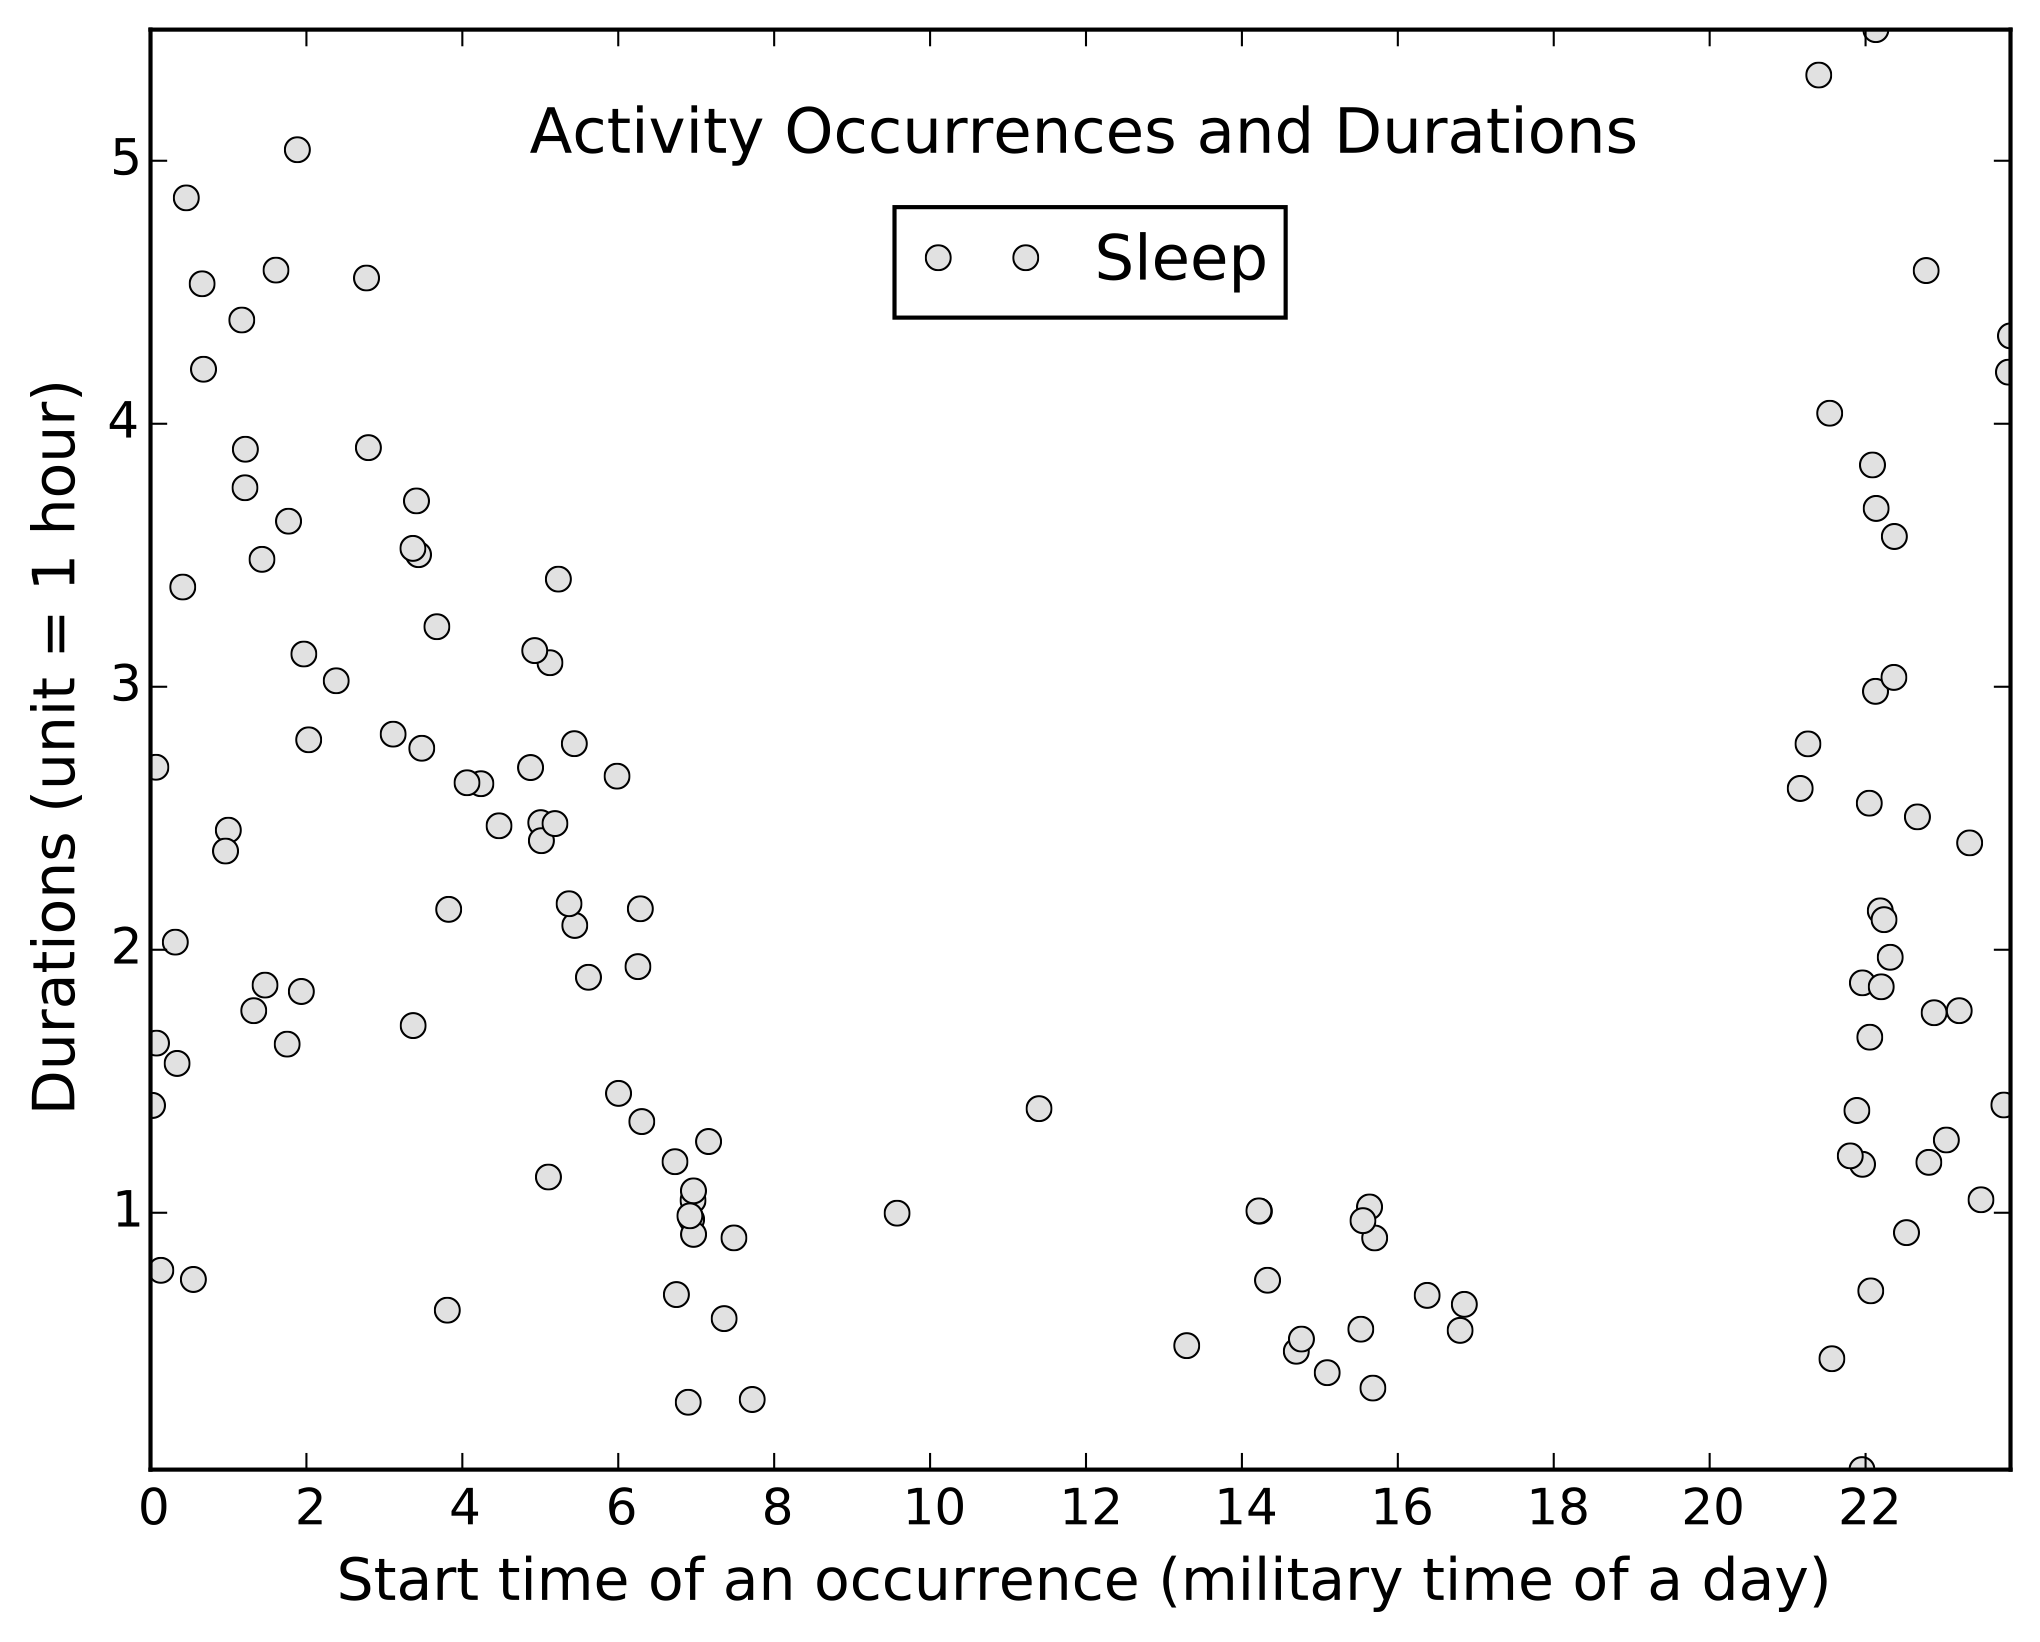
\includegraphics[width=\linewidth]{figures/adl_tm/Activity_time_stat_sleep_bw}
    \caption{Distribution of ``Sleep''}
    \label{fig:vissleep-b}
\end{subfigure}
 \caption{Topic 8 and Annotated Activity Sleep (dataset: hh122). The $x$-axis indicates the start time of a segment 
%  the format is military time so the range is 0:0:0 to 23:59:59, 
 and the $y$-axis gives the duration of a segment in hours.}
\label{fig:vissleep}
\end{figure}

%\setlength{\tabcolsep}{0.5em} % for the horizontal padding
{%\renewcommand{\arraystretch}{1.2}% for the vertical padding
\begin{table}[!b]
\centering
\scriptsize
\begin{tabular}{ccccccc}
\toprule
{\bf \begin{tabular}[c]{@{}c@{}}Sub-\\ Topic\end{tabular}} & {\bf \begin{tabular}[c]{@{}c@{}}Cook \\ Breakfast\end{tabular}} & {\bf \begin{tabular}[c]{@{}c@{}}Wash\\ Breakfast \\Dishes\end{tabular}} & {\bf \begin{tabular}[c]{@{}c@{}}Cook\\ Lunch\end{tabular}} & {\bf \begin{tabular}[c]{@{}c@{}}Wash\\ Lunch \\Dishes\end{tabular}} & {\bf \begin{tabular}[c]{@{}c@{}}Cook\\ Dinner\end{tabular}} & {\bf \begin{tabular}[c]{@{}c@{}}Wash\\ Dinner \\Dishes\end{tabular}} \\ 
\midrule
0 & 0.985 & 0.904 & 0     & 0     & 0     & 0     \\
1 & 0     & 0     & 0     & 0     & 0.969 & 0.979 \\
2 & 0     & 0.041 & 0.960 & 0.983 & 0     & 0     \\
\bottomrule
\end{tabular}
\caption{Mapping between sub-topics and activities. The columns do not add to 1 since the activities do not only map to topic 11.  }
\label{tab:submap}
\end{table}
}

However, not all topics map to one specific activity: \eg activities in the kitchen are usually divided into breakfast, lunch and dinner activities, which can be distinguished by the time of their occurrences. As the discovered topic 11 (\Cref{fig:adl_tm-11}) corresponds to kitchen activities, a very simple but effective approach to obtain those sub-topics is $K$-means clustering. The only feature we need is the start time of a segment, and the number of clusters $K$ is set to 3. To examine how accurate the clustering result is we mapped the annotated kitchen activities to the discovered sub-topics as in \Cref{tab:submap}. The sub-topics successfully represent breakfast, lunch and dinner activities and the categorisation is quite precise.

We can also easily detect outliers by deploying $z$-scores on the duration of all data points of a topic. In this way, one outlier of kitchen activities has been detected in dataset hh122. The corresponding raw data points are shown in \Cref{tab:outlier}: between the two sensors switching on then off no other sensor activations have occurred during more than 2 hours, which is clearly an abnormal situation.

%\setlength{\tabcolsep}{0.5em} % for the horizontal padding
{%\renewcommand{\arraystretch}{1.2}% for the vertical padding
\begin{table}[!t]
\centering
\scriptsize
\begin{tabular}{ccccc}
\toprule
{\bf Timestamp}            & {\bf Sensor} & {\bf Reading} & {\bf Location}  \\ 
\midrule
2013-04-27 18:29:28.187573 & MA011        & ON            & Kitchen              \\ 
2013-04-27 18:29:29.339714 & MA011        & OFF           & Kitchen               \\ 
2013-04-27 20:47:55.930002 & M010         & ON            & Kitchen               \\ 
2013-04-27 20:47:57.065529 & M010         & OFF           & Kitchen                \\ 
\bottomrule
\end{tabular}
\caption{A detected abnormal pattern.}
\label{tab:outlier}
\end{table}

%\input{sections/06_conclusions}
\section{Conclusions and Future Work}

In this paper we proposed a topic model \ac{ADLTM} and a segmentation algorithm for discovery of \acl{ADL} in a smart home. It is a novel unsupervised approach for modelling sequential sensor data, thus sidestepping the expensive requirement of providing labelled training data. Successful unsupervised methods are a crucial step in making activity discovery feasible in practice. 
% Our approach works as follows. 
% We first segment the sensor data into a set of documents by a location-based algorithm and then train \ac{ADLTM} on these documents to obtain latent topics that can be interpreted as activities. We treat a single sensor with a specific reading as one unigram word, and the transition between two unigram words as one bigram pair of words. 
% \ac{ADLTM} is able to discover the hidden structure of a document from both unigram and bigram words in parallel so that it can simulate the generative process of an actual activity more closely. 
Our experimental results have demonstrated that discovered topics can represent actual activities successfully and work effectively in various practical applications. The segmentation of the data is also close to the true segments with a low level of error. \ac{ADLTM} outperforms \acf{LDA} \cite{blei2003latent} and the \acf{BTM} \cite{wallach2006topic} in both criteria of the topic-activity similarity and segmentation evaluations.

There are several avenues for future work.
Simultaneously categorising data by spatial as well as temporal dimensions could enhance the clustering performance, some ideas have been introduced in topic models for document categorisation \cite{wang2006topics}\cite{wang2012continuous}.
Secondly, in order perform incremental discovery of new topics, an online extension of the model is required, which for efficiency would require an online variational inference algorithm as used for standard LDA \cite{hoffman2010online}.
Thirdly, since a small part of labelled data could provide prior knowledge that can be used for estimating hyperparameters and for mapping topics to actual activities, it is also worth extending the model to allow semi-supervised learning\cite{toutanova2007bayesian}.
%A more sophisticated algorithm for generating documents could consider the gap between two activities when segmenting the data. 
Finally, correlations between topics could be introduced into the model, following ideas proposed in \cite{blei2007correlated} and \cite{hospedales2009markov}. 


% TODO: uncomment if accepted
\subsubsection*{Acknowledgments}

This work was performed under the \ac{SPHERE} Inter\-disciplinary Research Collaboration funded by the UK Engineering and Physical Sciences Research Council, Grant EP/K031910/1.
\clearpage
\bibliographystyle{named}
{\small
\bibliography{bibghy2}}

\end{document}


